% Seminarul 3: Distribuții α-stabile
% Statistica piețelor financiare -- Program de licență, Academia de Studii Economice din București
% GENERAT de latex/build_seminar3.py -- modificați generatorul, nu acest fișier.
% Implicit versiunea pentru studenți; versiunea profesorului este wrapper-ul *_solutions.tex.
\makeatletter\@ifundefined{ifsolutions}{\expandafter\newif\csname ifsolutions\endcsname}{}\makeatother

\newcommand{\coursename}{Statistica piețelor financiare}
\def\sfmlang{ro}
% Preambul comun SFM -- Statistica piețelor financiare / Statistics of Financial Markets (Beamer, 16:9)
% Același design ca MFM. Înainte de % Preambul comun SFM -- Statistica piețelor financiare / Statistics of Financial Markets (Beamer, 16:9)
% Același design ca MFM. Înainte de % Preambul comun SFM -- Statistica piețelor financiare / Statistics of Financial Markets (Beamer, 16:9)
% Același design ca MFM. Înainte de \input{../../latex/preamble} se definește
%   \newcommand{\coursename}{Statistics of Financial Markets}      (EN)
%   \newcommand{\coursename}{Statistica piețelor financiare}       (RO)  și  \def\sfmlang{ro}
% Fișierele .tex se află în EN/Courses, EN/Seminars, RO/Cursuri, RO/Seminarii (două niveluri sub rădăcină).
% Deck-urile sînt generate de latex/build_chapterN.py / build_seminarN.py (vezi latex/sfm_build.py).

\documentclass[9pt, aspectratio=169, t]{beamer}
\providecommand{\coursename}{Statistics of Financial Markets}

% Ensure content fits on slides
\setbeamersize{text margin left=8mm, text margin right=8mm}

%=============================================================================
% THEME AND STYLE CONFIGURATION
%=============================================================================
\usetheme{default}
% Using default theme for clean header/footer control

% Color Palette (matching Redispatch PDF)
\definecolor{MainBlue}{RGB}{26, 58, 110}
\definecolor{AccentBlue}{RGB}{26, 58, 110}
\definecolor{IDAred}{RGB}{205, 0, 0}
\definecolor{DarkGray}{RGB}{51, 51, 51}
\definecolor{MediumGray}{RGB}{128, 128, 128}
\definecolor{LightGray}{RGB}{248, 248, 248}
\definecolor{VeryLightGray}{RGB}{235, 235, 235}
\definecolor{KeynoteGray}{RGB}{218, 218, 218}
\definecolor{SectionGray}{RGB}{120, 120, 120}
\definecolor{FooterGray}{RGB}{100, 100, 100}
\definecolor{Crimson}{RGB}{220, 53, 69}
\definecolor{Forest}{RGB}{46, 125, 50}
\definecolor{Amber}{RGB}{181, 133, 63}
\definecolor{Orange}{RGB}{230, 126, 34}
\definecolor{Purple}{RGB}{142, 68, 173}

% Gradient background (exact Keynote 315° gradient: white to RGB 218,218,218)
\setbeamertemplate{background}{%
    \begin{tikzpicture}[remember picture, overlay]
        \shade[shading=axis, shading angle=315,
        top color=white, bottom color=KeynoteGray]
        (current page.south west) rectangle (current page.north east);
    \end{tikzpicture}%
}
% Fallback solid color for compatibility
\setbeamercolor{background canvas}{bg=}

\setbeamercolor{palette primary}{bg=MainBlue, fg=white}
\setbeamercolor{palette secondary}{bg=MainBlue!85, fg=white}
\setbeamercolor{palette tertiary}{bg=MainBlue!70, fg=white}
\setbeamercolor{structure}{fg=MainBlue}
\setbeamercolor{title}{fg=IDAred}
\setbeamercolor{frametitle}{fg=IDAred, bg=}
\setbeamercolor{block title}{bg=MainBlue, fg=white}
\setbeamercolor{block body}{bg=VeryLightGray, fg=DarkGray}
\setbeamercolor{block title alerted}{bg=Crimson, fg=white}
\setbeamercolor{block body alerted}{bg=Crimson!8, fg=DarkGray}
\setbeamercolor{block title example}{bg=Forest, fg=white}
\setbeamercolor{block body example}{bg=Forest!8, fg=DarkGray}
\setbeamercolor{item}{fg=MainBlue}

% Footer colors (override Madrid theme blue)
\setbeamercolor{author in head/foot}{fg=FooterGray, bg=}
\setbeamercolor{title in head/foot}{fg=FooterGray, bg=}
\setbeamercolor{date in head/foot}{fg=FooterGray, bg=}
\setbeamercolor{section in head/foot}{fg=FooterGray, bg=}
\setbeamercolor{subsection in head/foot}{fg=FooterGray, bg=}

% Bullet styles (apply everywhere including blocks)
\setbeamertemplate{itemize item}{\color{MainBlue}$\boxdot$}
\setbeamertemplate{itemize subitem}{\color{MainBlue}$\blacktriangleright$}
\setbeamertemplate{itemize subsubitem}{\color{MainBlue}\tiny$\bullet$}
\setbeamertemplate{itemize/enumerate body begin}{\normalsize}
\setbeamertemplate{itemize/enumerate subbody begin}{\normalsize}

% Item spacing - compact style
\setlength{\leftmargini}{10pt}       % Level 1: minimal indent
\setlength{\leftmarginii}{10pt}      % Level 2: minimal additional indent
% Compact list spacing (zero extra space before/after lists in blocks)
\makeatletter
\def\@listi{\leftmargin\leftmargini \topsep 0pt \parsep 0pt \itemsep 0pt}
\def\@listii{\leftmargin\leftmarginii \topsep 0pt \parsep 0pt \itemsep 0pt}
\makeatother

\setbeamertemplate{navigation symbols}{}

%=============================================================================
% CUSTOM HEADLINE
%=============================================================================
\setbeamertemplate{headline}{%
    \vskip10pt%
    \hbox to \paperwidth{%
        \hskip0.5cm%
        {\small\color{FooterGray}\renewcommand{\hyperlink}[2]{##2}\insertsectionhead}%
        \hfill%
        \textcolor{FooterGray}{\small\insertframenumber}%
        \hskip0.5cm%
    }%
    \vskip4pt%
    {\color{FooterGray}\hrule height 0.4pt}%
}

%=============================================================================
% CUSTOM FOOTER
%=============================================================================
\usepackage{fontawesome5}

\setbeamertemplate{footline}{%
    {\color{FooterGray}\hrule height 0.4pt}%
    \vskip4pt%
    \hbox to \paperwidth{%
        \hskip0.5cm%
        \textcolor{FooterGray}{\small\coursename}%
        \hfill%
        \raisebox{-0.1em}{%
            \begin{tikzpicture}[x=0.08em, y=0.08em, line width=0.4pt]
                \draw[FooterGray] (0,3) -- (1,4) -- (2,3.5) -- (3,5) -- (4,4) -- (5,6) -- (6,5.5) -- (7,4) -- (8,5) -- (9,7) -- (10,6) -- (11,5) -- (12,6.5) -- (13,8) -- (14,7) -- (15,6) -- (16,7.5) -- (17,9) -- (18,8) -- (19,7) -- (20,8.5) -- (21,10) -- (22,9) -- (23,8) -- (24,9.5);
            \end{tikzpicture}%
        }%
        \hskip0.5cm%
    }%
    \vskip6pt%
}

%=============================================================================
% PACKAGES
%=============================================================================
\usepackage[utf8]{inputenc}
\DeclareUnicodeCharacter{03B1}{\ensuremath{\alpha}}
\usepackage[T1]{fontenc}
\usepackage{amsmath, amssymb, amsthm}
\usepackage{mathtools}
\usepackage{bm}
\usepackage{tikz}
\usetikzlibrary{arrows.meta, positioning, shapes, calc, decorations.pathreplacing, shadings}
\usepackage{booktabs}
\usepackage{multirow}
\usepackage{array}
\usepackage{graphicx}
\usepackage{hyperref}
\usepackage{colortbl}
\usepackage{listings}
\lstset{language=Python, basicstyle=\ttfamily\scriptsize, keywordstyle=\color{MainBlue}\bfseries,
  commentstyle=\color{Forest}, stringstyle=\color{Crimson}, breaklines=true,
  frame=none, backgroundcolor=\color{VeryLightGray}, xleftmargin=2mm}
\hypersetup{colorlinks=true, linkcolor=MainBlue, urlcolor=MainBlue}
\graphicspath{{../../logos/}{../../charts/}{../../photos/}}
\usepackage{xcolor}
\hfuzz=2pt  % Suppress tiny overfull warnings (<2pt)
\vfuzz=2pt  % Suppress tiny vertical overfull warnings (<2pt)

%=============================================================================
% QUANTLET COMMANDS
%   \quantlet{<displayed name>}{<url>}       (generic, compatible with the older SFM decks)
%   \sfmquantlet{Ch_05}{SFM_ch5_garch}       -> https://github.com/danpele/SFM/tree/main/Quantlets/Ch_05/SFM_ch5_garch
%   \qlurl{<folder>} is defined per chapter by the generator (Quantlets/Ch_NN/<folder>)
%=============================================================================
\newcommand{\sfmrepo}{https://github.com/danpele/SFM}
\newcommand{\sfmqlbase}{https://github.com/danpele/SFM/tree/main/Quantlets}
\newcommand{\quantlet}[2]{%
    \hfill\href{#2}{%
        \raisebox{-0.15em}{
\includegraphics[height=0.7em]{ql_logo.png}}%
        \textcolor{MainBlue}{\tiny\ #1}%
    }%
}
\newcommand{\sfmquantlet}[2]{\quantlet{\detokenize{#2}}{\sfmqlbase/#1/#2}}

%=============================================================================
% NOTEBOOKS (Google Colab)
%   \colaburl{notebooks/EN/chapter5_seminar_notebook.ipynb} -> the Colab link of a file in the SFM repo
%   \nb: the chapter notebook (each seminar deck redefines it with \renewcommand)
%=============================================================================
\newcommand{\colaburl}[1]{https://colab.research.google.com/github/danpele/SFM/blob/main/#1}
\newcommand{\nb}{https://colab.research.google.com/github/danpele/SFM/tree/main/notebooks/EN}
\newcommand{\nbname}{notebooks/EN}

%=============================================================================
% SLIDE HELPERS (used by the generators; the same as in MFM)
%=============================================================================
% local font size for list bodies (the preamble forces \normalsize)
\newcommand{\itemsize}[1]{\setbeamertemplate{itemize/enumerate body begin}{#1}\setbeamertemplate{itemize/enumerate subbody begin}{#1}}
\newcommand{\intitle}[1]{{\hypersetup{urlcolor=white}#1}}   % white links inside coloured title bars
\newcommand{\imgcap}[1]{{\scriptsize #1}\\[0.5mm]}          % caption under a photo
\newcommand{\imgcredit}[2]{{\tiny\color{FooterGray}\href{#1}{#2}}}   % image credit: source URL, author/licence
\newcommand{\aiprompt}[1]{{\ttfamily\color{MainBlue}#1}}     % a prompt to an AI assistant

%=============================================================================
% SEMINARS: student version by default; the instructor wrapper *_solutions.tex sets \solutionstrue
%=============================================================================
\makeatletter\@ifundefined{ifsolutions}{\expandafter\newif\csname ifsolutions\endcsname}{}\makeatother
\newcommand{\solonly}[1]{\ifsolutions #1\fi}
\newcommand{\propsub}{\ifsolutions\else\framesubtitle{\ifdefined\sfmlang Rezolvarea se discută la seminar\else Solution discussed in class\fi}\fi}

%=============================================================================
% APPENDIX AND CHAPTER LINKS (latex/appendix_links.py writes the calls; it also re-declares these
% macros before \begin{document}, so the decks compile with or without this preamble block)
%=============================================================================
\providecommand{\sfmapplink}[3]{\hypertarget{#2}{}\hyperlink{#1}{\beamergotobutton{#3}}}
\providecommand{\sfmappback}[2]{\begin{tikzpicture}[remember picture,overlay]\node[anchor=south east] at ([xshift=-3mm,yshift=7mm]current page.south east){\hyperlink{#1}{\beamerreturnbutton{#2}}};\end{tikzpicture}}
\providecommand{\sfmchlink}[2]{\href{#1}{#2}}
\providecommand{\sfmchlinkt}[2]{\href{#1}{\usebeamercolor[fg]{frametitle}#2}}

%=============================================================================
% QUANTINAR COMMAND: link către un curs Quantinar (subiecte avansate)
%=============================================================================
\newcommand{\quantinar}[2]{%
    \href{#2}{%
        \raisebox{-0.15em}{
\includegraphics[height=0.8em]{qr_logo.png}}%
        \textcolor{MainBlue}{\scriptsize\ #1}%
    }%
}

%=============================================================================
% CUSTOM TITLE PAGE
%=============================================================================
\defbeamertemplate*{title page}{hybrid}[1][]
{
    \vspace{0.2cm}
    % Logos row - top header (with clickable links)
    \begin{center}
        \href{https://www.ase.ro}{
\includegraphics[height=1.0cm]{ase_logo.png}}\hspace{0.3cm}%
        \href{https://theida.net}{
\includegraphics[height=1.0cm]{ida_logo.png}}\hspace{0.3cm}%
        \href{https://blockchain-research-center.com}{
\includegraphics[height=1.0cm]{brc_logo.png}}\hspace{0.3cm}%
        \href{https://www.ai4efin.ase.ro}{
\includegraphics[height=1.0cm]{ai4efin_logo.png}}\hspace{0.3cm}%
        \href{https://ipe.ro/new}{
\includegraphics[height=1.0cm]{acad_logo.png}}\hspace{0.3cm}%
        \href{https://www.digital-finance-msca.com}{
\includegraphics[height=1.0cm]{msca_logo.png}}%
    \end{center}

    \vspace{0.6cm}

    % Main title with Q logos on sides (with clickable links)
    \begin{center}
        \begin{minipage}{0.1\textwidth}
            \centering
            \href{https://quantlet.com}{
\includegraphics[height=1.1cm]{ql_logo.png}}
        \end{minipage}%
        \begin{minipage}{0.78\textwidth}
            \centering
            {\LARGE\bfseries\usebeamercolor[fg]{title}\inserttitle}

            \vspace{0.3cm}

            {\usebeamerfont{subtitle}\usebeamercolor[fg]{title}\insertsubtitle}
        \end{minipage}%
        \begin{minipage}{0.1\textwidth}
            \centering
            \href{https://quantinar.com}{
\includegraphics[height=1.1cm]{qr_logo.png}}
        \end{minipage}
    \end{center}

    \vspace{0.6cm}

    % Authors (left aligned)
    \hspace{0.5cm}{\usebeamerfont{author}\insertauthor}

    \vspace{0.3cm}

    % Institute/Affiliations (left aligned)
    \hspace{0.5cm}\begin{minipage}[t]{0.9\textwidth}
        \raggedright\small\insertinstitute
    \end{minipage}
}

%=============================================================================
% THEOREM ENVIRONMENTS
%=============================================================================
\theoremstyle{definition}
\setbeamertemplate{theorems}[numbered]
\ifdefined\sfmlang
\newtheorem{defn}{Definiție}
\newtheorem{thm}{Teoremă}
\newtheorem{prop}{Propoziție}
\newtheorem{rmk}{Observație}
\else
\newtheorem{defn}{Definition}
\newtheorem{thm}{Theorem}
\newtheorem{prop}{Proposition}
\newtheorem{rmk}{Remark}
\fi

%=============================================================================
% CENTRED MINIPAGE (no extra vertical space)
%=============================================================================
\newenvironment{cminipage}[1]{%
    \par\noindent\hfill\begin{minipage}{#1}\ignorespaces
}{%
    \end{minipage}\hfill\null\par
}

%=============================================================================
% CUSTOM COMMANDS
%=============================================================================
\newcommand{\E}{\mathbb{E}}
\newcommand{\Var}{\text{Var}}
\newcommand{\Cov}{\text{Cov}}
\newcommand{\Corr}{\text{Corr}}
\newcommand{\R}{\mathbb{R}}
\newcommand{\N}{\mathbb{N}}
\newcommand{\Z}{\mathbb{Z}}
\newcommand{\B}{\mathbf{B}}
\newcommand{\imark}{\textcolor{MainBlue}{\textbullet}}
\newcommand{\RMSE}{\text{RMSE}}
\newcommand{\MAE}{\text{MAE}}
\newcommand{\MAPE}{\text{MAPE}}

 se definește
%   \newcommand{\coursename}{Statistics of Financial Markets}      (EN)
%   \newcommand{\coursename}{Statistica piețelor financiare}       (RO)  și  \def\sfmlang{ro}
% Fișierele .tex se află în EN/Courses, EN/Seminars, RO/Cursuri, RO/Seminarii (două niveluri sub rădăcină).
% Deck-urile sînt generate de latex/build_chapterN.py / build_seminarN.py (vezi latex/sfm_build.py).

\documentclass[9pt, aspectratio=169, t]{beamer}
\providecommand{\coursename}{Statistics of Financial Markets}

% Ensure content fits on slides
\setbeamersize{text margin left=8mm, text margin right=8mm}

%=============================================================================
% THEME AND STYLE CONFIGURATION
%=============================================================================
\usetheme{default}
% Using default theme for clean header/footer control

% Color Palette (matching Redispatch PDF)
\definecolor{MainBlue}{RGB}{26, 58, 110}
\definecolor{AccentBlue}{RGB}{26, 58, 110}
\definecolor{IDAred}{RGB}{205, 0, 0}
\definecolor{DarkGray}{RGB}{51, 51, 51}
\definecolor{MediumGray}{RGB}{128, 128, 128}
\definecolor{LightGray}{RGB}{248, 248, 248}
\definecolor{VeryLightGray}{RGB}{235, 235, 235}
\definecolor{KeynoteGray}{RGB}{218, 218, 218}
\definecolor{SectionGray}{RGB}{120, 120, 120}
\definecolor{FooterGray}{RGB}{100, 100, 100}
\definecolor{Crimson}{RGB}{220, 53, 69}
\definecolor{Forest}{RGB}{46, 125, 50}
\definecolor{Amber}{RGB}{181, 133, 63}
\definecolor{Orange}{RGB}{230, 126, 34}
\definecolor{Purple}{RGB}{142, 68, 173}

% Gradient background (exact Keynote 315° gradient: white to RGB 218,218,218)
\setbeamertemplate{background}{%
    \begin{tikzpicture}[remember picture, overlay]
        \shade[shading=axis, shading angle=315,
        top color=white, bottom color=KeynoteGray]
        (current page.south west) rectangle (current page.north east);
    \end{tikzpicture}%
}
% Fallback solid color for compatibility
\setbeamercolor{background canvas}{bg=}

\setbeamercolor{palette primary}{bg=MainBlue, fg=white}
\setbeamercolor{palette secondary}{bg=MainBlue!85, fg=white}
\setbeamercolor{palette tertiary}{bg=MainBlue!70, fg=white}
\setbeamercolor{structure}{fg=MainBlue}
\setbeamercolor{title}{fg=IDAred}
\setbeamercolor{frametitle}{fg=IDAred, bg=}
\setbeamercolor{block title}{bg=MainBlue, fg=white}
\setbeamercolor{block body}{bg=VeryLightGray, fg=DarkGray}
\setbeamercolor{block title alerted}{bg=Crimson, fg=white}
\setbeamercolor{block body alerted}{bg=Crimson!8, fg=DarkGray}
\setbeamercolor{block title example}{bg=Forest, fg=white}
\setbeamercolor{block body example}{bg=Forest!8, fg=DarkGray}
\setbeamercolor{item}{fg=MainBlue}

% Footer colors (override Madrid theme blue)
\setbeamercolor{author in head/foot}{fg=FooterGray, bg=}
\setbeamercolor{title in head/foot}{fg=FooterGray, bg=}
\setbeamercolor{date in head/foot}{fg=FooterGray, bg=}
\setbeamercolor{section in head/foot}{fg=FooterGray, bg=}
\setbeamercolor{subsection in head/foot}{fg=FooterGray, bg=}

% Bullet styles (apply everywhere including blocks)
\setbeamertemplate{itemize item}{\color{MainBlue}$\boxdot$}
\setbeamertemplate{itemize subitem}{\color{MainBlue}$\blacktriangleright$}
\setbeamertemplate{itemize subsubitem}{\color{MainBlue}\tiny$\bullet$}
\setbeamertemplate{itemize/enumerate body begin}{\normalsize}
\setbeamertemplate{itemize/enumerate subbody begin}{\normalsize}

% Item spacing - compact style
\setlength{\leftmargini}{10pt}       % Level 1: minimal indent
\setlength{\leftmarginii}{10pt}      % Level 2: minimal additional indent
% Compact list spacing (zero extra space before/after lists in blocks)
\makeatletter
\def\@listi{\leftmargin\leftmargini \topsep 0pt \parsep 0pt \itemsep 0pt}
\def\@listii{\leftmargin\leftmarginii \topsep 0pt \parsep 0pt \itemsep 0pt}
\makeatother

\setbeamertemplate{navigation symbols}{}

%=============================================================================
% CUSTOM HEADLINE
%=============================================================================
\setbeamertemplate{headline}{%
    \vskip10pt%
    \hbox to \paperwidth{%
        \hskip0.5cm%
        {\small\color{FooterGray}\renewcommand{\hyperlink}[2]{##2}\insertsectionhead}%
        \hfill%
        \textcolor{FooterGray}{\small\insertframenumber}%
        \hskip0.5cm%
    }%
    \vskip4pt%
    {\color{FooterGray}\hrule height 0.4pt}%
}

%=============================================================================
% CUSTOM FOOTER
%=============================================================================
\usepackage{fontawesome5}

\setbeamertemplate{footline}{%
    {\color{FooterGray}\hrule height 0.4pt}%
    \vskip4pt%
    \hbox to \paperwidth{%
        \hskip0.5cm%
        \textcolor{FooterGray}{\small\coursename}%
        \hfill%
        \raisebox{-0.1em}{%
            \begin{tikzpicture}[x=0.08em, y=0.08em, line width=0.4pt]
                \draw[FooterGray] (0,3) -- (1,4) -- (2,3.5) -- (3,5) -- (4,4) -- (5,6) -- (6,5.5) -- (7,4) -- (8,5) -- (9,7) -- (10,6) -- (11,5) -- (12,6.5) -- (13,8) -- (14,7) -- (15,6) -- (16,7.5) -- (17,9) -- (18,8) -- (19,7) -- (20,8.5) -- (21,10) -- (22,9) -- (23,8) -- (24,9.5);
            \end{tikzpicture}%
        }%
        \hskip0.5cm%
    }%
    \vskip6pt%
}

%=============================================================================
% PACKAGES
%=============================================================================
\usepackage[utf8]{inputenc}
\DeclareUnicodeCharacter{03B1}{\ensuremath{\alpha}}
\usepackage[T1]{fontenc}
\usepackage{amsmath, amssymb, amsthm}
\usepackage{mathtools}
\usepackage{bm}
\usepackage{tikz}
\usetikzlibrary{arrows.meta, positioning, shapes, calc, decorations.pathreplacing, shadings}
\usepackage{booktabs}
\usepackage{multirow}
\usepackage{array}
\usepackage{graphicx}
\usepackage{hyperref}
\usepackage{colortbl}
\usepackage{listings}
\lstset{language=Python, basicstyle=\ttfamily\scriptsize, keywordstyle=\color{MainBlue}\bfseries,
  commentstyle=\color{Forest}, stringstyle=\color{Crimson}, breaklines=true,
  frame=none, backgroundcolor=\color{VeryLightGray}, xleftmargin=2mm}
\hypersetup{colorlinks=true, linkcolor=MainBlue, urlcolor=MainBlue}
\graphicspath{{../../logos/}{../../charts/}{../../photos/}}
\usepackage{xcolor}
\hfuzz=2pt  % Suppress tiny overfull warnings (<2pt)
\vfuzz=2pt  % Suppress tiny vertical overfull warnings (<2pt)

%=============================================================================
% QUANTLET COMMANDS
%   \quantlet{<displayed name>}{<url>}       (generic, compatible with the older SFM decks)
%   \sfmquantlet{Ch_05}{SFM_ch5_garch}       -> https://github.com/danpele/SFM/tree/main/Quantlets/Ch_05/SFM_ch5_garch
%   \qlurl{<folder>} is defined per chapter by the generator (Quantlets/Ch_NN/<folder>)
%=============================================================================
\newcommand{\sfmrepo}{https://github.com/danpele/SFM}
\newcommand{\sfmqlbase}{https://github.com/danpele/SFM/tree/main/Quantlets}
\newcommand{\quantlet}[2]{%
    \hfill\href{#2}{%
        \raisebox{-0.15em}{
\includegraphics[height=0.7em]{ql_logo.png}}%
        \textcolor{MainBlue}{\tiny\ #1}%
    }%
}
\newcommand{\sfmquantlet}[2]{\quantlet{\detokenize{#2}}{\sfmqlbase/#1/#2}}

%=============================================================================
% NOTEBOOKS (Google Colab)
%   \colaburl{notebooks/EN/chapter5_seminar_notebook.ipynb} -> the Colab link of a file in the SFM repo
%   \nb: the chapter notebook (each seminar deck redefines it with \renewcommand)
%=============================================================================
\newcommand{\colaburl}[1]{https://colab.research.google.com/github/danpele/SFM/blob/main/#1}
\newcommand{\nb}{https://colab.research.google.com/github/danpele/SFM/tree/main/notebooks/EN}
\newcommand{\nbname}{notebooks/EN}

%=============================================================================
% SLIDE HELPERS (used by the generators; the same as in MFM)
%=============================================================================
% local font size for list bodies (the preamble forces \normalsize)
\newcommand{\itemsize}[1]{\setbeamertemplate{itemize/enumerate body begin}{#1}\setbeamertemplate{itemize/enumerate subbody begin}{#1}}
\newcommand{\intitle}[1]{{\hypersetup{urlcolor=white}#1}}   % white links inside coloured title bars
\newcommand{\imgcap}[1]{{\scriptsize #1}\\[0.5mm]}          % caption under a photo
\newcommand{\imgcredit}[2]{{\tiny\color{FooterGray}\href{#1}{#2}}}   % image credit: source URL, author/licence
\newcommand{\aiprompt}[1]{{\ttfamily\color{MainBlue}#1}}     % a prompt to an AI assistant

%=============================================================================
% SEMINARS: student version by default; the instructor wrapper *_solutions.tex sets \solutionstrue
%=============================================================================
\makeatletter\@ifundefined{ifsolutions}{\expandafter\newif\csname ifsolutions\endcsname}{}\makeatother
\newcommand{\solonly}[1]{\ifsolutions #1\fi}
\newcommand{\propsub}{\ifsolutions\else\framesubtitle{\ifdefined\sfmlang Rezolvarea se discută la seminar\else Solution discussed in class\fi}\fi}

%=============================================================================
% APPENDIX AND CHAPTER LINKS (latex/appendix_links.py writes the calls; it also re-declares these
% macros before \begin{document}, so the decks compile with or without this preamble block)
%=============================================================================
\providecommand{\sfmapplink}[3]{\hypertarget{#2}{}\hyperlink{#1}{\beamergotobutton{#3}}}
\providecommand{\sfmappback}[2]{\begin{tikzpicture}[remember picture,overlay]\node[anchor=south east] at ([xshift=-3mm,yshift=7mm]current page.south east){\hyperlink{#1}{\beamerreturnbutton{#2}}};\end{tikzpicture}}
\providecommand{\sfmchlink}[2]{\href{#1}{#2}}
\providecommand{\sfmchlinkt}[2]{\href{#1}{\usebeamercolor[fg]{frametitle}#2}}

%=============================================================================
% QUANTINAR COMMAND: link către un curs Quantinar (subiecte avansate)
%=============================================================================
\newcommand{\quantinar}[2]{%
    \href{#2}{%
        \raisebox{-0.15em}{
\includegraphics[height=0.8em]{qr_logo.png}}%
        \textcolor{MainBlue}{\scriptsize\ #1}%
    }%
}

%=============================================================================
% CUSTOM TITLE PAGE
%=============================================================================
\defbeamertemplate*{title page}{hybrid}[1][]
{
    \vspace{0.2cm}
    % Logos row - top header (with clickable links)
    \begin{center}
        \href{https://www.ase.ro}{
\includegraphics[height=1.0cm]{ase_logo.png}}\hspace{0.3cm}%
        \href{https://theida.net}{
\includegraphics[height=1.0cm]{ida_logo.png}}\hspace{0.3cm}%
        \href{https://blockchain-research-center.com}{
\includegraphics[height=1.0cm]{brc_logo.png}}\hspace{0.3cm}%
        \href{https://www.ai4efin.ase.ro}{
\includegraphics[height=1.0cm]{ai4efin_logo.png}}\hspace{0.3cm}%
        \href{https://ipe.ro/new}{
\includegraphics[height=1.0cm]{acad_logo.png}}\hspace{0.3cm}%
        \href{https://www.digital-finance-msca.com}{
\includegraphics[height=1.0cm]{msca_logo.png}}%
    \end{center}

    \vspace{0.6cm}

    % Main title with Q logos on sides (with clickable links)
    \begin{center}
        \begin{minipage}{0.1\textwidth}
            \centering
            \href{https://quantlet.com}{
\includegraphics[height=1.1cm]{ql_logo.png}}
        \end{minipage}%
        \begin{minipage}{0.78\textwidth}
            \centering
            {\LARGE\bfseries\usebeamercolor[fg]{title}\inserttitle}

            \vspace{0.3cm}

            {\usebeamerfont{subtitle}\usebeamercolor[fg]{title}\insertsubtitle}
        \end{minipage}%
        \begin{minipage}{0.1\textwidth}
            \centering
            \href{https://quantinar.com}{
\includegraphics[height=1.1cm]{qr_logo.png}}
        \end{minipage}
    \end{center}

    \vspace{0.6cm}

    % Authors (left aligned)
    \hspace{0.5cm}{\usebeamerfont{author}\insertauthor}

    \vspace{0.3cm}

    % Institute/Affiliations (left aligned)
    \hspace{0.5cm}\begin{minipage}[t]{0.9\textwidth}
        \raggedright\small\insertinstitute
    \end{minipage}
}

%=============================================================================
% THEOREM ENVIRONMENTS
%=============================================================================
\theoremstyle{definition}
\setbeamertemplate{theorems}[numbered]
\ifdefined\sfmlang
\newtheorem{defn}{Definiție}
\newtheorem{thm}{Teoremă}
\newtheorem{prop}{Propoziție}
\newtheorem{rmk}{Observație}
\else
\newtheorem{defn}{Definition}
\newtheorem{thm}{Theorem}
\newtheorem{prop}{Proposition}
\newtheorem{rmk}{Remark}
\fi

%=============================================================================
% CENTRED MINIPAGE (no extra vertical space)
%=============================================================================
\newenvironment{cminipage}[1]{%
    \par\noindent\hfill\begin{minipage}{#1}\ignorespaces
}{%
    \end{minipage}\hfill\null\par
}

%=============================================================================
% CUSTOM COMMANDS
%=============================================================================
\newcommand{\E}{\mathbb{E}}
\newcommand{\Var}{\text{Var}}
\newcommand{\Cov}{\text{Cov}}
\newcommand{\Corr}{\text{Corr}}
\newcommand{\R}{\mathbb{R}}
\newcommand{\N}{\mathbb{N}}
\newcommand{\Z}{\mathbb{Z}}
\newcommand{\B}{\mathbf{B}}
\newcommand{\imark}{\textcolor{MainBlue}{\textbullet}}
\newcommand{\RMSE}{\text{RMSE}}
\newcommand{\MAE}{\text{MAE}}
\newcommand{\MAPE}{\text{MAPE}}

 se definește
%   \newcommand{\coursename}{Statistics of Financial Markets}      (EN)
%   \newcommand{\coursename}{Statistica piețelor financiare}       (RO)  și  \def\sfmlang{ro}
% Fișierele .tex se află în EN/Courses, EN/Seminars, RO/Cursuri, RO/Seminarii (două niveluri sub rădăcină).
% Deck-urile sînt generate de latex/build_chapterN.py / build_seminarN.py (vezi latex/sfm_build.py).

\documentclass[9pt, aspectratio=169, t]{beamer}
\providecommand{\coursename}{Statistics of Financial Markets}

% Ensure content fits on slides
\setbeamersize{text margin left=8mm, text margin right=8mm}

%=============================================================================
% THEME AND STYLE CONFIGURATION
%=============================================================================
\usetheme{default}
% Using default theme for clean header/footer control

% Color Palette (matching Redispatch PDF)
\definecolor{MainBlue}{RGB}{26, 58, 110}
\definecolor{AccentBlue}{RGB}{26, 58, 110}
\definecolor{IDAred}{RGB}{205, 0, 0}
\definecolor{DarkGray}{RGB}{51, 51, 51}
\definecolor{MediumGray}{RGB}{128, 128, 128}
\definecolor{LightGray}{RGB}{248, 248, 248}
\definecolor{VeryLightGray}{RGB}{235, 235, 235}
\definecolor{KeynoteGray}{RGB}{218, 218, 218}
\definecolor{SectionGray}{RGB}{120, 120, 120}
\definecolor{FooterGray}{RGB}{100, 100, 100}
\definecolor{Crimson}{RGB}{220, 53, 69}
\definecolor{Forest}{RGB}{46, 125, 50}
\definecolor{Amber}{RGB}{181, 133, 63}
\definecolor{Orange}{RGB}{230, 126, 34}
\definecolor{Purple}{RGB}{142, 68, 173}

% Gradient background (exact Keynote 315° gradient: white to RGB 218,218,218)
\setbeamertemplate{background}{%
    \begin{tikzpicture}[remember picture, overlay]
        \shade[shading=axis, shading angle=315,
        top color=white, bottom color=KeynoteGray]
        (current page.south west) rectangle (current page.north east);
    \end{tikzpicture}%
}
% Fallback solid color for compatibility
\setbeamercolor{background canvas}{bg=}

\setbeamercolor{palette primary}{bg=MainBlue, fg=white}
\setbeamercolor{palette secondary}{bg=MainBlue!85, fg=white}
\setbeamercolor{palette tertiary}{bg=MainBlue!70, fg=white}
\setbeamercolor{structure}{fg=MainBlue}
\setbeamercolor{title}{fg=IDAred}
\setbeamercolor{frametitle}{fg=IDAred, bg=}
\setbeamercolor{block title}{bg=MainBlue, fg=white}
\setbeamercolor{block body}{bg=VeryLightGray, fg=DarkGray}
\setbeamercolor{block title alerted}{bg=Crimson, fg=white}
\setbeamercolor{block body alerted}{bg=Crimson!8, fg=DarkGray}
\setbeamercolor{block title example}{bg=Forest, fg=white}
\setbeamercolor{block body example}{bg=Forest!8, fg=DarkGray}
\setbeamercolor{item}{fg=MainBlue}

% Footer colors (override Madrid theme blue)
\setbeamercolor{author in head/foot}{fg=FooterGray, bg=}
\setbeamercolor{title in head/foot}{fg=FooterGray, bg=}
\setbeamercolor{date in head/foot}{fg=FooterGray, bg=}
\setbeamercolor{section in head/foot}{fg=FooterGray, bg=}
\setbeamercolor{subsection in head/foot}{fg=FooterGray, bg=}

% Bullet styles (apply everywhere including blocks)
\setbeamertemplate{itemize item}{\color{MainBlue}$\boxdot$}
\setbeamertemplate{itemize subitem}{\color{MainBlue}$\blacktriangleright$}
\setbeamertemplate{itemize subsubitem}{\color{MainBlue}\tiny$\bullet$}
\setbeamertemplate{itemize/enumerate body begin}{\normalsize}
\setbeamertemplate{itemize/enumerate subbody begin}{\normalsize}

% Item spacing - compact style
\setlength{\leftmargini}{10pt}       % Level 1: minimal indent
\setlength{\leftmarginii}{10pt}      % Level 2: minimal additional indent
% Compact list spacing (zero extra space before/after lists in blocks)
\makeatletter
\def\@listi{\leftmargin\leftmargini \topsep 0pt \parsep 0pt \itemsep 0pt}
\def\@listii{\leftmargin\leftmarginii \topsep 0pt \parsep 0pt \itemsep 0pt}
\makeatother

\setbeamertemplate{navigation symbols}{}

%=============================================================================
% CUSTOM HEADLINE
%=============================================================================
\setbeamertemplate{headline}{%
    \vskip10pt%
    \hbox to \paperwidth{%
        \hskip0.5cm%
        {\small\color{FooterGray}\renewcommand{\hyperlink}[2]{##2}\insertsectionhead}%
        \hfill%
        \textcolor{FooterGray}{\small\insertframenumber}%
        \hskip0.5cm%
    }%
    \vskip4pt%
    {\color{FooterGray}\hrule height 0.4pt}%
}

%=============================================================================
% CUSTOM FOOTER
%=============================================================================
\usepackage{fontawesome5}

\setbeamertemplate{footline}{%
    {\color{FooterGray}\hrule height 0.4pt}%
    \vskip4pt%
    \hbox to \paperwidth{%
        \hskip0.5cm%
        \textcolor{FooterGray}{\small\coursename}%
        \hfill%
        \raisebox{-0.1em}{%
            \begin{tikzpicture}[x=0.08em, y=0.08em, line width=0.4pt]
                \draw[FooterGray] (0,3) -- (1,4) -- (2,3.5) -- (3,5) -- (4,4) -- (5,6) -- (6,5.5) -- (7,4) -- (8,5) -- (9,7) -- (10,6) -- (11,5) -- (12,6.5) -- (13,8) -- (14,7) -- (15,6) -- (16,7.5) -- (17,9) -- (18,8) -- (19,7) -- (20,8.5) -- (21,10) -- (22,9) -- (23,8) -- (24,9.5);
            \end{tikzpicture}%
        }%
        \hskip0.5cm%
    }%
    \vskip6pt%
}

%=============================================================================
% PACKAGES
%=============================================================================
\usepackage[utf8]{inputenc}
\DeclareUnicodeCharacter{03B1}{\ensuremath{\alpha}}
\usepackage[T1]{fontenc}
\usepackage{amsmath, amssymb, amsthm}
\usepackage{mathtools}
\usepackage{bm}
\usepackage{tikz}
\usetikzlibrary{arrows.meta, positioning, shapes, calc, decorations.pathreplacing, shadings}
\usepackage{booktabs}
\usepackage{multirow}
\usepackage{array}
\usepackage{graphicx}
\usepackage{hyperref}
\usepackage{colortbl}
\usepackage{listings}
\lstset{language=Python, basicstyle=\ttfamily\scriptsize, keywordstyle=\color{MainBlue}\bfseries,
  commentstyle=\color{Forest}, stringstyle=\color{Crimson}, breaklines=true,
  frame=none, backgroundcolor=\color{VeryLightGray}, xleftmargin=2mm}
\hypersetup{colorlinks=true, linkcolor=MainBlue, urlcolor=MainBlue}
\graphicspath{{../../logos/}{../../charts/}{../../photos/}}
\usepackage{xcolor}
\hfuzz=2pt  % Suppress tiny overfull warnings (<2pt)
\vfuzz=2pt  % Suppress tiny vertical overfull warnings (<2pt)

%=============================================================================
% QUANTLET COMMANDS
%   \quantlet{<displayed name>}{<url>}       (generic, compatible with the older SFM decks)
%   \sfmquantlet{Ch_05}{SFM_ch5_garch}       -> https://github.com/danpele/SFM/tree/main/Quantlets/Ch_05/SFM_ch5_garch
%   \qlurl{<folder>} is defined per chapter by the generator (Quantlets/Ch_NN/<folder>)
%=============================================================================
\newcommand{\sfmrepo}{https://github.com/danpele/SFM}
\newcommand{\sfmqlbase}{https://github.com/danpele/SFM/tree/main/Quantlets}
\newcommand{\quantlet}[2]{%
    \hfill\href{#2}{%
        \raisebox{-0.15em}{
\includegraphics[height=0.7em]{ql_logo.png}}%
        \textcolor{MainBlue}{\tiny\ #1}%
    }%
}
\newcommand{\sfmquantlet}[2]{\quantlet{\detokenize{#2}}{\sfmqlbase/#1/#2}}

%=============================================================================
% NOTEBOOKS (Google Colab)
%   \colaburl{notebooks/EN/chapter5_seminar_notebook.ipynb} -> the Colab link of a file in the SFM repo
%   \nb: the chapter notebook (each seminar deck redefines it with \renewcommand)
%=============================================================================
\newcommand{\colaburl}[1]{https://colab.research.google.com/github/danpele/SFM/blob/main/#1}
\newcommand{\nb}{https://colab.research.google.com/github/danpele/SFM/tree/main/notebooks/EN}
\newcommand{\nbname}{notebooks/EN}

%=============================================================================
% SLIDE HELPERS (used by the generators; the same as in MFM)
%=============================================================================
% local font size for list bodies (the preamble forces \normalsize)
\newcommand{\itemsize}[1]{\setbeamertemplate{itemize/enumerate body begin}{#1}\setbeamertemplate{itemize/enumerate subbody begin}{#1}}
\newcommand{\intitle}[1]{{\hypersetup{urlcolor=white}#1}}   % white links inside coloured title bars
\newcommand{\imgcap}[1]{{\scriptsize #1}\\[0.5mm]}          % caption under a photo
\newcommand{\imgcredit}[2]{{\tiny\color{FooterGray}\href{#1}{#2}}}   % image credit: source URL, author/licence
\newcommand{\aiprompt}[1]{{\ttfamily\color{MainBlue}#1}}     % a prompt to an AI assistant

%=============================================================================
% SEMINARS: student version by default; the instructor wrapper *_solutions.tex sets \solutionstrue
%=============================================================================
\makeatletter\@ifundefined{ifsolutions}{\expandafter\newif\csname ifsolutions\endcsname}{}\makeatother
\newcommand{\solonly}[1]{\ifsolutions #1\fi}
\newcommand{\propsub}{\ifsolutions\else\framesubtitle{\ifdefined\sfmlang Rezolvarea se discută la seminar\else Solution discussed in class\fi}\fi}

%=============================================================================
% APPENDIX AND CHAPTER LINKS (latex/appendix_links.py writes the calls; it also re-declares these
% macros before \begin{document}, so the decks compile with or without this preamble block)
%=============================================================================
\providecommand{\sfmapplink}[3]{\hypertarget{#2}{}\hyperlink{#1}{\beamergotobutton{#3}}}
\providecommand{\sfmappback}[2]{\begin{tikzpicture}[remember picture,overlay]\node[anchor=south east] at ([xshift=-3mm,yshift=7mm]current page.south east){\hyperlink{#1}{\beamerreturnbutton{#2}}};\end{tikzpicture}}
\providecommand{\sfmchlink}[2]{\href{#1}{#2}}
\providecommand{\sfmchlinkt}[2]{\href{#1}{\usebeamercolor[fg]{frametitle}#2}}

%=============================================================================
% QUANTINAR COMMAND: link către un curs Quantinar (subiecte avansate)
%=============================================================================
\newcommand{\quantinar}[2]{%
    \href{#2}{%
        \raisebox{-0.15em}{
\includegraphics[height=0.8em]{qr_logo.png}}%
        \textcolor{MainBlue}{\scriptsize\ #1}%
    }%
}

%=============================================================================
% CUSTOM TITLE PAGE
%=============================================================================
\defbeamertemplate*{title page}{hybrid}[1][]
{
    \vspace{0.2cm}
    % Logos row - top header (with clickable links)
    \begin{center}
        \href{https://www.ase.ro}{
\includegraphics[height=1.0cm]{ase_logo.png}}\hspace{0.3cm}%
        \href{https://theida.net}{
\includegraphics[height=1.0cm]{ida_logo.png}}\hspace{0.3cm}%
        \href{https://blockchain-research-center.com}{
\includegraphics[height=1.0cm]{brc_logo.png}}\hspace{0.3cm}%
        \href{https://www.ai4efin.ase.ro}{
\includegraphics[height=1.0cm]{ai4efin_logo.png}}\hspace{0.3cm}%
        \href{https://ipe.ro/new}{
\includegraphics[height=1.0cm]{acad_logo.png}}\hspace{0.3cm}%
        \href{https://www.digital-finance-msca.com}{
\includegraphics[height=1.0cm]{msca_logo.png}}%
    \end{center}

    \vspace{0.6cm}

    % Main title with Q logos on sides (with clickable links)
    \begin{center}
        \begin{minipage}{0.1\textwidth}
            \centering
            \href{https://quantlet.com}{
\includegraphics[height=1.1cm]{ql_logo.png}}
        \end{minipage}%
        \begin{minipage}{0.78\textwidth}
            \centering
            {\LARGE\bfseries\usebeamercolor[fg]{title}\inserttitle}

            \vspace{0.3cm}

            {\usebeamerfont{subtitle}\usebeamercolor[fg]{title}\insertsubtitle}
        \end{minipage}%
        \begin{minipage}{0.1\textwidth}
            \centering
            \href{https://quantinar.com}{
\includegraphics[height=1.1cm]{qr_logo.png}}
        \end{minipage}
    \end{center}

    \vspace{0.6cm}

    % Authors (left aligned)
    \hspace{0.5cm}{\usebeamerfont{author}\insertauthor}

    \vspace{0.3cm}

    % Institute/Affiliations (left aligned)
    \hspace{0.5cm}\begin{minipage}[t]{0.9\textwidth}
        \raggedright\small\insertinstitute
    \end{minipage}
}

%=============================================================================
% THEOREM ENVIRONMENTS
%=============================================================================
\theoremstyle{definition}
\setbeamertemplate{theorems}[numbered]
\ifdefined\sfmlang
\newtheorem{defn}{Definiție}
\newtheorem{thm}{Teoremă}
\newtheorem{prop}{Propoziție}
\newtheorem{rmk}{Observație}
\else
\newtheorem{defn}{Definition}
\newtheorem{thm}{Theorem}
\newtheorem{prop}{Proposition}
\newtheorem{rmk}{Remark}
\fi

%=============================================================================
% CENTRED MINIPAGE (no extra vertical space)
%=============================================================================
\newenvironment{cminipage}[1]{%
    \par\noindent\hfill\begin{minipage}{#1}\ignorespaces
}{%
    \end{minipage}\hfill\null\par
}

%=============================================================================
% CUSTOM COMMANDS
%=============================================================================
\newcommand{\E}{\mathbb{E}}
\newcommand{\Var}{\text{Var}}
\newcommand{\Cov}{\text{Cov}}
\newcommand{\Corr}{\text{Corr}}
\newcommand{\R}{\mathbb{R}}
\newcommand{\N}{\mathbb{N}}
\newcommand{\Z}{\mathbb{Z}}
\newcommand{\B}{\mathbf{B}}
\newcommand{\imark}{\textcolor{MainBlue}{\textbullet}}
\newcommand{\RMSE}{\text{RMSE}}
\newcommand{\MAE}{\text{MAE}}
\newcommand{\MAPE}{\text{MAPE}}



\newcommand{\qlurl}[1]{https://github.com/danpele/SFM/tree/main/Quantlets/Ch_03/#1}
\renewcommand{\nb}{\colaburl{notebooks/EN/chapter3_seminar_notebook.ipynb}}
\renewcommand{\nbname}{chapter3\_seminar\_notebook.ipynb}
% left column: full width in the student version, narrower next to the solution
\newcommand{\taskw}{\ifsolutions 0.47\textwidth\else 0.96\textwidth\fi}
\newcommand{\solw}{\ifsolutions 0.49\textwidth\else 0pt\fi}

\DeclareUnicodeCharacter{03B1}{\ensuremath{\alpha}}

% Clickable citations (DOIs verified via Crossref)

\newcommand{\refMandelbrot}{\href{https://doi.org/10.1086/294632}{Mandelbrot (1963)}}
\newcommand{\refFama}{\href{https://doi.org/10.1086/294743}{Fama (1965)}}
\newcommand{\refFamaRoll}{\href{https://doi.org/10.1080/01621459.1968.11009311}{Fama \& Roll (1968)}}
\newcommand{\refFamaRollB}{\href{https://doi.org/10.1080/01621459.1971.10482264}{Fama \& Roll (1971)}}
\newcommand{\refCMS}{\href{https://doi.org/10.1080/01621459.1976.10480344}{Chambers, Mallows \& Stuck (1976)}}
\newcommand{\refWeron}{\href{https://doi.org/10.1016/0167-7152(95)00113-1}{Weron (1996)}}
\newcommand{\refMcCulloch}{\href{https://doi.org/10.1080/03610918608812563}{McCulloch (1986)}}
\newcommand{\refNolanA}{\href{https://doi.org/10.1080/15326349708807450}{Nolan (1997)}}
\newcommand{\refNolan}{\href{https://doi.org/10.1007/978-3-030-52915-4}{Nolan (2020)}}
\newcommand{\refNolanML}{\href{https://doi.org/10.1007/978-1-4612-0197-7_17}{Nolan (2001)}}
\newcommand{\refST}{\href{https://doi.org/10.1201/9780203738818}{Samorodnitsky \& Taqqu (1994)}}
\newcommand{\refBHW}{\href{https://doi.org/10.1007/3-540-27395-6_1}{Borak, Härdle \& Weron (2005)}}
\newcommand{\refBMW}{\href{https://doi.org/10.1007/978-3-642-18062-0_1}{Borak, Misiorek \& Weron (2011)}}
\newcommand{\refFHH}{\href{https://doi.org/10.1007/978-3-030-13751-9}{Franke, Härdle \& Hafner (2019)}}
\newcommand{\refOfficer}{\href{https://doi.org/10.1080/01621459.1972.10481297}{Officer (1972)}}
\newcommand{\refBG}{\href{https://doi.org/10.1086/295634}{Blattberg \& Gonedes (1974)}}
\newcommand{\refAB}{\href{https://doi.org/10.1080/07350015.1988.10509636}{Akgiray \& Booth (1988)}}
\newcommand{\refLLW}{\href{https://doi.org/10.1080/07350015.1990.10509793}{Lau, Lau \& Wingender (1990)}}
\newcommand{\refCont}{\href{https://doi.org/10.1080/713665670}{Cont (2001)}}
\newcommand{\refRM}{\href{https://www.wiley.com/en-us/Stable+Paretian+Models+in+Finance-p-9780471953142}{Rachev \& Mittnik (2000)}}
\newcommand{\refMDC}{\href{https://doi.org/10.1016/S0895-7177(99)00106-5}{Mittnik, Doganoglu \& Chenyao (1999)}}
\newcommand{\refMRDC}{\href{https://doi.org/10.1016/S0895-7177(99)00110-7}{Mittnik et al.\ (1999)}}
\newcommand{\refKoutrouvelis}{\href{https://doi.org/10.1080/01621459.1980.10477573}{Koutrouvelis (1980)}}
\newcommand{\refMS}{\href{https://doi.org/10.1038/376046a0}{Mantegna \& Stanley (1995)}}
\newcommand{\refGopi}{\href{https://doi.org/10.1103/PhysRevE.60.5305}{Gopikrishnan et al.\ (1999)}}
\newcommand{\refWang}{\href{https://doi.org/10.1038/s41586-023-06221-2}{Wang et al.\ (2023)}}
\newcommand{\refGS}{\href{https://doi.org/10.1080/14697680903540381}{Grabchak \& Samorodnitsky (2010)}}
\newcommand{\refHill}{\href{https://doi.org/10.1214/aos/1176343247}{Hill (1975)}}
\newcommand{\refGK}{\href{https://archive.org/details/limitdistributio00gned_0}{Gnedenko \& Kolmogorov (1954)}}
\newcommand{\refPele}{\href{https://doi.org/10.1016/S2212-5671(14)00279-2}{Pele (2014)}}

\title[Statistica piețelor financiare]{Statistica piețelor financiare}
\subtitle{Seminarul 3: Distribuții α-stabile\ifsolutions\ (versiunea profesorului)\fi}
\author[D.T. Pele]{Daniel Traian PELE}
\institute{Academia de Studii Economice din București\\
IDA Institute Digital Assets\\
Blockchain Research Center\\
AI4EFin Artificial Intelligence for Energy Finance\\
Academia Română, Institutul de Prognoză Economică\\
MSCA Digital Finance}
\date{}

%=============================================================================
\providecommand{\sfmapplink}[3]{\hypertarget{#2}{}\hyperlink{#1}{\beamergotobutton{#3}}}  % APPLINKS-MACROS
\providecommand{\sfmappback}[2]{\begin{tikzpicture}[remember picture,overlay]\node[anchor=south east] at ([xshift=-3mm,yshift=7mm]current page.south east){\hyperlink{#1}{\beamerreturnbutton{#2}}};\end{tikzpicture}}  % APPLINKS-MACROS
\providecommand{\sfmchlink}[2]{\href{#1}{#2}}  % APPLINKS-MACROS
\providecommand{\sfmchlinkt}[2]{\href{#1}{\usebeamercolor[fg]{frametitle}#2}}  % APPLINKS-MACROS
\begin{document}
%=============================================================================

{
\setbeamertemplate{headline}{}
\setbeamertemplate{footline}{}
\begin{frame}[noframenumbering]
    \titlepage
\end{frame}
}
% BEGIN-ACRONYMS (generat de latex/acronyms.py; nu editati manual)
\begin{frame}{Acronime folosite în acest material}
\setbeamertemplate{itemize/enumerate body begin}{\tiny}
\begin{columns}[T]
\begin{column}{0.49\textwidth}
\begin{itemize}\setlength{\itemsep}{0pt}
    \item \textbf{AI}: Artificial Intelligence (inteligență artificială)
    \item \textbf{AIC}: Akaike Information Criterion (criteriul informațional Akaike)
    \item \textbf{BET}: Bucharest Exchange Trading (index) (indicele de referință al Bursei de Valori București)
    \item \textbf{BVB}: Bursa de Valori București
    \item \textbf{CI}: Confidence Interval (interval de încredere)
    \item \textbf{CLT}: Central Limit Theorem (teorema limită centrală)
    \item \textbf{CMS}: Chambers–Mallows–Stuck (simulation method) (metoda de simulare Chambers–Mallows–Stuck)
    \item \textbf{EODHD}: EOD Historical Data (market-data provider) (furnizor de date de piață)
    \item \textbf{ES}: Expected Shortfall (pierderea așteptată în coadă)
    \item \textbf{GARCH}: Generalised AutoRegressive Conditional Heteroskedasticity (heteroscedasticitate condiționată autoregresivă generalizată)
    \item \textbf{GCLT}: Generalised Central Limit Theorem (teorema limită centrală generalizată)
    \item \textbf{ML}: Maximum Likelihood (verosimilitate maximă)
    \item \textbf{QQ}: Quantile–Quantile (plot) (graficul cuantilă–cuantilă)
\end{itemize}
\end{column}
\begin{column}{0.49\textwidth}
\begin{itemize}\setlength{\itemsep}{0pt}
    \item \textbf{SE}: Standard Error (eroare standard)
\end{itemize}
\end{column}
\end{columns}
\end{frame}
% END-ACRONYMS

\begin{frame}{Întrebarea de azi și traseul}
\itemsize{\small}
\begin{itemize}
    \item \textbf{Întrebarea}: poate o lege stabilă cu $\alpha < 2$ să descrie randamentele zilnice și ce implică ea despre sumele lor?
    \begin{itemize}
        \item seminarul are loc \textbf{înaintea} Cursului 3: secțiunea „Ce vă trebuie azi” dă toate definițiile folosite în cerințe
    \end{itemize}
    \item Traseul
    \begin{itemize}
        \item Partea A: stabilitate, funcții caracteristice, cozi, tabelele McCulloch și o extragere simulată, pe hîrtie
        \item Partea B: ajustări stabile pe randamentele BET, S\&P 500, DAX și Bitcoin, fiecare cu o măsură a preciziei și o întrebare de interpretare
        \item Partea C: o întrebare deschisă pentru proiect și un răspuns AI de verificat
    \end{itemize}
    \item Notebook-ul de azi: \href{\nb}{deschideți notebook-ul seminarului în Google Colab}; fiecare cerință indică secțiunea din notebook
    \item Nu se predă nimic: seminarul este pentru exercițiu; rezolvările cerințelor [Propus] se discută la seminar
\end{itemize}
\end{frame}

\begin{frame}{Harta exercițiilor}
\itemsize{\small}
\begin{center}
\footnotesize
\begin{tabular}{>{\raggedright\arraybackslash}p{1.1cm}>{\raggedright\arraybackslash}p{7.5cm}>{\raggedright\arraybackslash}p{1.9cm}>{\raggedright\arraybackslash}p{1.4cm}}
\toprule
\textbf{Cerința} & \textbf{Întrebarea} & \textbf{Tipul} & \textbf{Model} \\
\midrule
A1, A2 & cum crește scala unei sume cu numărul de termeni? & Rezolvat, Propus & A1 \\
A3, A4 & ce se schimbă între parametrizările S1 și S0? & Rezolvat, Propus & A3 \\
A5, A6 & cît de repede scad cozile de tip putere? & Rezolvat, Propus & A5 \\
A7, A8 & estimări McCulloch din cinci cuantile & Rezolvat, Propus & A7 \\
A9, A10 & o extragere stabilă prin metoda CMS & Rezolvat, Propus & A9 \\
B1, B2 & cît de groase sînt cozile randamentelor BET, S\&P 500, DAX și Bitcoin? & Rezolvat, Propus & B1 \\
B3, B4 & ajustare ML, grafic QQ, pierderi mari: stabilă vs Normală vs Student-t & Rezolvat, Propus & B3 \\
B5, B6 & rămîne $\alpha$ la fel pentru randamentele săptămînale și lunare? se stabilizează varianța? & Rezolvat, Propus & B5 \\
C1, C2 & este $\alpha$ constant în timp? ce este greșit într-un răspuns AI? & Propus & B1, B3 \\
\bottomrule
\end{tabular}
\end{center}
\begin{itemize}
    \item \textbf{[Rezolvat]}: rezolvarea completă în slide-uri și în notebook, un model de urmat; \textbf{[Propus]}: îl rezolvați voi, după model
\end{itemize}
\end{frame}

\begin{frame}{Datele folosite}
\itemsize{\small}
\begin{center}
\footnotesize
\begin{tabular}{llll}
\toprule
\textbf{Seria} & \textbf{Sursa} & \textbf{Prețul folosit} & \textbf{Perioada} \\
\midrule
BET, S\&P 500, DAX & EODHD & close & 2000--2026 \\
Bitcoin & EODHD & close, 7 zile pe săptămînă & 2014--2026 \\
\bottomrule
\end{tabular}
\end{center}
\begin{itemize}
    \item Randamente logaritmice zilnice în \%: $r_t = 100\,(\ln P_t - \ln P_{t-1})$; weekendurile și închiderile repetate din zilele libere se elimină (cu excepția Bitcoin)
    \item Randamente logaritmice săptămînale și lunare: sumele randamentelor logaritmice zilnice din fiecare săptămînă sau lună calendaristică
    \item În notebook: \texttt{log\_returns('bet', '2000-01-01')}; nu este nevoie de cont sau de cheie
\end{itemize}
\end{frame}


%=============================================================================
\section{Ce vă trebuie azi}
%=============================================================================

\begin{frame}{Ce vă trebuie azi (1/5): legi stabile și sume}
\itemsize{\small}
\begin{itemize}
    \item $X$ este \textbf{stabilă} dacă, pentru copii independente $X_1, X_2$ și orice $a, b > 0$: $aX_1 + bX_2 \overset{d}{=} cX + d$ ($\overset{d}{=}$: aceeași distribuție)
    \begin{itemize}
        \item regula scalei: $c^\alpha = a^\alpha + b^\alpha$, cu \textbf{indicele de stabilitate} $0 < \alpha \le 2$
        \item $n$ copii independente: $X_1 + \dots + X_n \overset{d}{=} n^{1/\alpha}X + d_n$
    \end{itemize}
    \item Exemple
    \begin{itemize}
        \item Normală ($\alpha = 2$): varianțele se adună, $c^2 = a^2 + b^2$
        \item Cauchy ($\alpha = 1$, densitatea $1/(\pi(1 + x^2))$): scalele se adună, $c = a + b$
    \end{itemize}
    \item \textbf{GCLT} (teorema limită centrală generalizată): legile stabile sînt singurele limite posibile ale sumelor normalizate de variabile i.i.d.\ (independente și identic distribuite); cu varianță finită, limita este Normală
\end{itemize}
\end{frame}

\begin{frame}{Ce vă trebuie azi (2/5): parametri și parametrizări}
\itemsize{\small}
\begin{itemize}
    \item \textbf{Funcția caracteristică} $\varphi(t) = E[e^{itX}]$; există întotdeauna și definește legea
    \begin{itemize}
        \item S1, $\alpha \ne 1$: $\ln\varphi(t) = -\gamma^\alpha|t|^\alpha\big[1 - i\beta\,\mathrm{sign}(t)\tan\frac{\pi\alpha}{2}\big] + i\delta_1 t$
        \item S0, $\alpha \ne 1$: $\ln\varphi(t) = -\gamma^\alpha|t|^\alpha\big[1 + i\beta\,\mathrm{sign}(t)\tan\frac{\pi\alpha}{2}(|\gamma t|^{1-\alpha} - 1)\big] + i\delta_0 t$
    \end{itemize}
    \item Parametri: $\alpha$ cozi, $\beta \in [-1, 1]$ asimetrie, $\gamma > 0$ scală, $\delta$ locație; diferă doar locația: $\delta_0 = \delta_1 + \beta\gamma\tan\frac{\pi\alpha}{2}$
    \item Cazuri particulare și capcane
    \begin{itemize}
        \item $\alpha = 2$: $N(\delta, 2\gamma^2)$, varianța $2\gamma^2$; $\alpha = 1$, $\beta = 0$: Cauchy, $\varphi(t) = e^{-\gamma|t| + i\delta t}$
        \item \texttt{scipy.stats.levy\_stable} folosește implicit S1 (\texttt{loc} $= \delta_1$, \texttt{scale} $= \gamma$)
    \end{itemize}
\end{itemize}
\end{frame}

\begin{frame}{Ce vă trebuie azi (3/5): cozi și momente}
\itemsize{\small}
\begin{itemize}
    \item Pentru $\alpha < 2$, cozi de tip putere: $P(X > x) \approx C x^{-\alpha}$ pentru $x$ mare
    \begin{itemize}
        \item deci $P(X > kx)/P(X > x) \approx k^{-\alpha}$: dublarea pragului împarte probabilitatea la $2^\alpha$
        \item coada distribuției Normale scade mult mai repede, ca $e^{-x^2/(2\sigma^2)}$
    \end{itemize}
    \item Momente: pentru $\alpha < 2$, $E|X|^p < \infty$ doar dacă $p < \alpha$
    \begin{itemize}
        \item $\alpha < 2$: varianță infinită; $\alpha \le 1$: nu există media; în S1, media ($\alpha > 1$) este $\delta_1$
        \item varianța de selecție a unui eșantion stabil continuă să sară pe măsură ce eșantionul crește
    \end{itemize}
    \item Cuantilele există întotdeauna: $\mathrm{VaR}_{1\%} = -q_{1\%}$, pierderea depășită cu probabilitatea 1\%; ES (expected shortfall) cere $\alpha > 1$
\end{itemize}
\end{frame}

\begin{frame}{Ce vă trebuie azi (4/5): simulare și estimare}
\itemsize{\small}
\begin{itemize}
    \item \textbf{CMS} (Chambers--Mallows--Stuck) pentru $S(\alpha; 0; 1; 0)$: $V = \pi(U - \frac12)$ cu $U \sim U(0, 1)$, $W \sim \mathrm{Exp}(1)$
    \begin{itemize}
        \item $X = \dfrac{\sin(\alpha V)}{(\cos V)^{1/\alpha}}\Big(\dfrac{\cos((1-\alpha)V)}{W}\Big)^{(1-\alpha)/\alpha}$; apoi $\gamma X + \delta$
    \end{itemize}
    \item \textbf{McCulloch} (1986): $\nu_\alpha = \dfrac{q_{0{,}95} - q_{0{,}05}}{q_{0{,}75} - q_{0{,}25}}$, $\nu_\beta = \dfrac{q_{0{,}95} + q_{0{,}05} - 2q_{0{,}5}}{q_{0{,}95} - q_{0{,}05}}$
    \begin{itemize}
        \item tabelele dau $\hat\alpha$, $\hat\beta$; apoi $\hat\gamma = (q_{0{,}75} - q_{0{,}25})/\phi_3(\hat\alpha, \hat\beta)$; Normală: $\nu_\alpha = 2{,}439$
    \end{itemize}
    \item \textbf{ML} (verosimilitate maximă): maximizați $\sum_t \ln f(r_t; \alpha, \beta, \gamma, \delta)$, cu $f$ calculat numeric din $\varphi$; erorile standard din curbură
    \item \textbf{Bootstrap}: reeșantionați zilele cu întoarcere de $B$ ori, reestimați de fiecare dată; percentilele de 2,5\% și 97,5\% dau un interval de 95\%
\end{itemize}
\end{frame}

\begin{frame}{Ce vă trebuie azi (5/5): tabelele McCulloch (extras)}
\itemsize{\footnotesize}
\begin{columns}[T]
\begin{column}{0.40\textwidth}
\begin{center}
\footnotesize
\begin{tabular}{rr}
\toprule
$\nu_\alpha$ & $\alpha$ \\
\midrule
$2{,}439$ & $2{,}000$ \\
$2{,}6$ & $1{,}808$ \\
$2{,}8$ & $1{,}664$ \\
$3{,}0$ & $1{,}563$ \\
$3{,}2$ & $1{,}484$ \\
$3{,}5$ & $1{,}391$ \\
$4{,}0$ & $1{,}279$ \\
$5{,}0$ & $1{,}128$ \\
$6{,}0$ & $1{,}029$ \\
\bottomrule
\end{tabular}
\end{center}

\end{column}
\begin{column}{0.56\textwidth}
\begin{center}
\footnotesize
\begin{tabular}{rr}
\toprule
$\alpha$ & $\phi_3(\alpha, 0)$ \\
\midrule
$2{,}0$ & $1{,}908$ \\
$1{,}8$ & $1{,}921$ \\
$1{,}6$ & $1{,}933$ \\
$1{,}5$ & $1{,}939$ \\
$1{,}4$ & $1{,}946$ \\
$1{,}3$ & $1{,}955$ \\
$1{,}2$ & $1{,}965$ \\
$1{,}1$ & $1{,}980$ \\
$1{,}0$ & $2{,}000$ \\
\bottomrule
\end{tabular}
\end{center}
\begin{itemize}
    \item Stînga: Tabelul III, coloana $\nu_\beta = 0$; dreapta: Tabelul V, coloana $\beta = 0$ \refMcCulloch
    \item Între două rînduri, interpolați liniar
    \item Pentru $|\nu_\beta| < 0{,}05$, coloanele cu $\beta = 0$ sînt suficient de apropiate pe hîrtie
\end{itemize}
\end{column}
\end{columns}
\end{frame}


%=============================================================================
\section{Partea A: calcule pe hîrtie}
%=============================================================================

\begin{frame}{A1: scala unei sume [Rezolvat]}
\itemsize{\footnotesize}
\begin{columns}[T]
\begin{column}{0.47\textwidth}
\begin{block}{Cerință}
\begin{itemize}
    \item $X_1, X_2$ sînt copii independente ale lui $S(\alpha; 0; 1; 0)$; $a = 3$, $b = 4$.
    \item 1. Calculați $c$ cu $3X_1 + 4X_2 \overset{d}{=} cX$ pentru $\alpha = 2$, $\alpha = 1{,}5$ și $\alpha = 1$.
    \item 2. Pentru $\alpha = 2$, verificați rezultatul cu varianțe.
    \item 3. Explicați de ce $c$ crește cînd $\alpha$ scade.
    \item Raportați: trei valori ale lui $c$ și o frază.
\end{itemize}
\end{block}
\end{column}
\begin{column}{0.49\textwidth}
\begin{exampleblock}{Rezolvare}
\begin{itemize}
    \item 1. $c = (3^\alpha + 4^\alpha)^{1/\alpha}$: $\alpha = 2$: $5{,}00$; $\alpha = 1{,}5$: $5{,}58$; $\alpha = 1$: $7{,}00$
    \item 2. $S(2; 0; 1; 0) = N(0, 2)$: $\mathrm{Var}(3X_1 + 4X_2) = (9 + 16) \cdot 2 = 50 = \mathrm{Var}(5X)$
    \item 3. Cu $\alpha$ mic, valorile mari sînt frecvente și un singur termen poate domina: scala sumei se apropie de suma scalelor.
\end{itemize}
\end{exampleblock}
\end{column}
\end{columns}
\end{frame}

\begin{frame}{A2: orizonturi și diversificare [Propus]}
\propsub
\itemsize{\footnotesize}
\begin{columns}[T]
\begin{column}{\taskw}
\begin{block}{Cerință}
\begin{itemize}
    \item Randamentele zilnice sînt i.i.d.\ $S(\alpha; 0; \gamma; 0)$. Model: A1.
    \item 1. Calculați scala sumei pe 20 de zile, ca multiplu al lui $\gamma$, pentru $\alpha = 2$, $1{,}7$ și $1{,}5$.
    \item 2. Calculați scala unui portofoliu cu ponderi egale din $N = 10$ active i.i.d.\ pentru $\alpha = 2$, $1{,}5$ și $1$.
    \item 3. Explicați ce se întîmplă cu diversificarea cînd $\alpha = 1$.
    \item Raportați: șase multipli ai lui $\gamma$ și o frază.
\end{itemize}
\end{block}
\end{column}
\begin{column}{\solw}
\solonly{%
\begin{exampleblock}{Rezolvare}
\begin{itemize}
    \item 1. $20^{1/\alpha}$: $4{,}47$, $5{,}83$, $7{,}37$
    \item 2. $\frac{1}{N}\sum_i X_i$ are scala $N^{1/\alpha - 1}\gamma$: $0{,}32$, $0{,}46$, $1{,}00$
    \item 3. Cu $\alpha = 1$, portofoliul are aceeași scală ca un singur activ: diversificarea nu reduce riscul.
\end{itemize}
\end{exampleblock}
}
\end{column}
\end{columns}
\end{frame}

\begin{frame}{A3: S1 și S0 în $t = 1$ [Rezolvat]}
\itemsize{\footnotesize}
\begin{columns}[T]
\begin{column}{0.47\textwidth}
\begin{block}{Cerință}
\begin{itemize}
    \item $X$ are $\alpha = 1{,}5$, $\beta = 0{,}3$, $\gamma = 1$, $\delta = 0$.
    \item 1. Calculați $\varphi(1)$ în parametrizarea S1.
    \item 2. Calculați $\varphi(1)$ în parametrizarea S0.
    \item 3. Explicați diferența folosind $\delta_0 = \delta_1 + \beta\gamma\tan\frac{\pi\alpha}{2}$.
    \item Raportați: două numere complexe și o frază.
\end{itemize}
\end{block}
\end{column}
\begin{column}{0.49\textwidth}
\begin{exampleblock}{Rezolvare}
\begin{itemize}
    \item 1. $\tan\frac{3\pi}{4} = -1{,}0$; $\ln\varphi(1) = -[1 - i(0{,}3)(-1)] = -1 - 0{,}3i$; $\varphi(1) = e^{-1}(\cos 0{,}3 - i\sin 0{,}3) = 0{,}351 - 0{,}109i$
    \item 2. $|t|^{1-\alpha} - 1 = 0$ în $t = 1$: $\varphi(1) = e^{-1} = 0{,}368$
    \item 3. Același modul $e^{-1}$; legile diferă printr-o deplasare: S1 cu $\delta_1 = 0$ este S0 cu $\delta_0 = 0{,}3 \cdot (-1{,}0) = -0{,}3$.
\end{itemize}
\end{exampleblock}
\end{column}
\end{columns}
\end{frame}

\begin{frame}{A4: cazuri particulare și o conversie a locației [Propus]}
\propsub
\itemsize{\footnotesize}
\begin{columns}[T]
\begin{column}{\taskw}
\begin{block}{Cerință}
\begin{itemize}
    \item Model: A3.
    \item 1. Scrieți $\varphi(t)$ pentru $\alpha = 2$ și comparați cu $\exp(i\mu t - \sigma^2 t^2/2)$, funcția caracteristică a $N(\mu, \sigma^2)$: cît sînt $\mu$ și $\sigma^2$?
    \item 2. Scrieți $\varphi(t)$ pentru $\alpha = 1$, $\beta = 0$ și numiți legea.
    \item 3. scipy raportează $\alpha = 1{,}7$, $\beta = -0{,}2$, $\gamma = 0{,}6$, \texttt{loc} $= 0{,}05$; calculați $\delta_0$.
    \item Raportați: $\mu$, $\sigma^2$, numele legii și $\delta_0$.
\end{itemize}
\end{block}
\end{column}
\begin{column}{\solw}
\solonly{%
\begin{exampleblock}{Rezolvare}
\begin{itemize}
    \item 1. $\varphi(t) = \exp(-\gamma^2 t^2 + i\delta t)$: $\mu = \delta$, $\sigma^2 = 2\gamma^2$ ($\beta$ nu contează, $\tan\pi = 0$)
    \item 2. $\varphi(t) = \exp(-\gamma|t| + i\delta t)$: legea Cauchy cu locația $\delta$ și scala $\gamma$
    \item 3. scipy folosește S1: $\delta_0 = 0{,}05 + (-0{,}2)(0{,}6)\tan(0{,}85\pi)$, $\tan(0{,}85\pi) = -0{,}5095$, deci $\delta_0 = 0{,}05 + 0{,}0611 = 0{,}111$
\end{itemize}
\end{exampleblock}
}
\end{column}
\end{columns}
\end{frame}

\begin{frame}{A5: cît de repede scad cozile? [Rezolvat]}
\itemsize{\footnotesize}
\begin{columns}[T]
\begin{column}{0.47\textwidth}
\begin{block}{Cerință}
\begin{itemize}
    \item Pierderile zilnice au o coadă de tip putere cu $\alpha = 1{,}7$; o pierdere peste $x$ apare într-o zi din 50.
    \item 1. Calculați $P(L > 2x)/P(L > x)$.
    \item 2. Cît de des apare o pierdere peste $2x$? Dar peste $4x$?
    \item 3. Comparați cu o lege Normală care are aceeași frecvență a pierderilor peste $x$.
    \item Raportați: un raport, două frecvențe și o frază.
\end{itemize}
\end{block}
\end{column}
\begin{column}{0.49\textwidth}
\begin{exampleblock}{Rezolvare}
\begin{itemize}
    \item 1. $2^{-1{,}7} = 0{,}308$
    \item 2. Peste $2x$: o zi din $50 \cdot 2^{1{,}7} \approx 162$; peste $4x$: o zi din $50 \cdot 4^{1{,}7} \approx 528$
    \item 3. Normală: $x = z_{0{,}98}\sigma$; $P(L > 2x) = P(Z > 2z_{0{,}98})$, adică o zi din circa $50\,004$: legea putere păstrează pierderile mari frecvente.
\end{itemize}
\end{exampleblock}
\end{column}
\end{columns}
\end{frame}

\begin{frame}{A6: cozi și momente pentru alte valori ale lui $\alpha$ [Propus]}
\propsub
\itemsize{\footnotesize}
\begin{columns}[T]
\begin{column}{\taskw}
\begin{block}{Cerință}
\begin{itemize}
    \item O pierdere peste $x$ apare într-o zi din 100. Model: A5.
    \item 1. Pentru $\alpha = 1{,}3$ și $\alpha = 1{,}9$, calculați cît de des apar pierderi peste $2x$ și peste $3x$.
    \item 2. Pentru $\alpha = 1{,}9$, $1{,}3$ și $0{,}8$, spuneți dacă există media și varianța.
    \item 3. Explicați de ce se poate calcula o varianță de selecție chiar dacă varianța nu există.
    \item Raportați: patru frecvențe, un mic tabel al momentelor și o frază.
\end{itemize}
\end{block}
\end{column}
\begin{column}{\solw}
\solonly{%
\begin{exampleblock}{Rezolvare}
\begin{itemize}
    \item 1. $\alpha = 1{,}3$: 1 din $246$ ($2x$), 1 din $417$ ($3x$); $\alpha = 1{,}9$: 1 din $373$, 1 din $806$
    \item 2. $\alpha = 1{,}9$ și $1{,}3$: media da, varianța nu; $\alpha = 0{,}8$: niciuna
    \item 3. Orice eșantion finit are o varianță de selecție finită; doar că ea nu converge către un număr cînd $n$ crește.
\end{itemize}
\end{exampleblock}
}
\end{column}
\end{columns}
\end{frame}

\begin{frame}{A7: McCulloch din cinci cuantile [Rezolvat]}
\itemsize{\scriptsize}
\begin{columns}[T]
\begin{column}{0.47\textwidth}
\begin{block}{Cerință}
\begin{itemize}
    \item Cuantilele a 2000 de randamente zilnice (\%): $q_{0{,}05} = -2{,}10$, $q_{0{,}25} = -0{,}55$, $q_{0{,}5} = 0{,}05$, $q_{0{,}75} = 0{,}62$, $q_{0{,}95} = 2{,}06$.
    \item 1. Calculați $\nu_\alpha$ și $\nu_\beta$.
    \item 2. Citiți $\hat\alpha$ din extrasul de tabel (coloana $\nu_\beta = 0$).
    \item 3. Calculați $\hat\gamma$ cu Tabelul V.
    \item Raportați: două rapoarte, $\hat\alpha$, $\hat\gamma$ și o frază despre cozi.
\end{itemize}
\end{block}
\end{column}
\begin{column}{0.49\textwidth}
\begin{exampleblock}{Rezolvare}
\begin{itemize}
    \item 1. $\nu_\alpha = 4{,}16/1{,}17 = 3{,}556$; $\nu_\beta = (2{,}06 - 2{,}10 - 0{,}10)/4{,}16 = -0{,}034$, aproape simetric
    \item 2. Între $3{,}5 \mapsto 1{,}391$ și $4{,}0 \mapsto 1{,}279$: $\hat\alpha \approx 1{,}379$
    \item 3. $\phi_3(\hat\alpha, 0) \approx 1{,}948$, deci $\hat\gamma = 1{,}17/1{,}948 = 0{,}601$
    \item Cu tabelele complete ($\nu_\beta \ne 0$): $\hat\alpha = 1{,}377$, $\hat\beta = -0{,}054$, $\hat\gamma = 0{,}599$; cozi mult mai groase decît la distribuția Normală ($\nu_\alpha = 2{,}439$).
\end{itemize}
\end{exampleblock}
\end{column}
\end{columns}
\end{frame}

\begin{frame}{A8: McCulloch pentru un activ cripto [Propus]}
\propsub
\itemsize{\scriptsize}
\begin{columns}[T]
\begin{column}{\taskw}
\begin{block}{Cerință}
\begin{itemize}
    \item Cuantilele randamentelor zilnice (\%): $q_{0{,}05} = -6{,}90$, $q_{0{,}25} = -1{,}45$, $q_{0{,}5} = 0{,}12$, $q_{0{,}75} = 1{,}75$, $q_{0{,}95} = 6{,}40$. Model: A7.
    \item 1. Calculați $\nu_\alpha$ și $\nu_\beta$.
    \item 2. Citiți $\hat\alpha$ și calculați $\hat\gamma$ din extrasele de tabel.
    \item 3. Comparați cu A7: care activ are cozile mai groase?
    \item Raportați: două rapoarte, $\hat\alpha$, $\hat\gamma$ și o frază.
\end{itemize}
\end{block}
\end{column}
\begin{column}{\solw}
\solonly{%
\begin{exampleblock}{Rezolvare}
\begin{itemize}
    \item 1. $\nu_\alpha = 13{,}30/3{,}20 = 4{,}156$; $\nu_\beta = -0{,}056$
    \item 2. Între $4{,}0 \mapsto 1{,}279$ și $5{,}0 \mapsto 1{,}128$: $\hat\alpha \approx 1{,}255$; $\phi_3 \approx 1{,}959$, $\hat\gamma \approx 1{,}633$ (tabelele complete: $1{,}252$, $1{,}624$)
    \item 3. Activul cripto: $\nu_\alpha$ mai mare, $\hat\alpha$ mai mic, cozi mai groase și o scală de aproape trei ori mai mare.
\end{itemize}
\end{exampleblock}
}
\end{column}
\end{columns}
\end{frame}

\begin{frame}{A9: o extragere stabilă prin CMS [Rezolvat]}
\itemsize{\footnotesize}
\begin{columns}[T]
\begin{column}{0.47\textwidth}
\begin{block}{Cerință}
\begin{itemize}
    \item $\alpha = 1{,}5$, $\beta = 0$; o extragere uniformă $U = 0{,}8$ și o extragere exponențială $W = 1{,}2$.
    \item 1. Calculați $V = \pi(U - 1/2)$.
    \item 2. Calculați cei trei factori ai formulei CMS.
    \item 3. Calculați extragerea $X$ și extragerea din $S(1{,}5; 0; 0{,}6; 0{,}05)$.
    \item Raportați: $V$, trei factori, două extrageri.
\end{itemize}
\end{block}
\end{column}
\begin{column}{0.49\textwidth}
\begin{exampleblock}{Rezolvare}
\begin{itemize}
    \item 1. $V = 0{,}3\pi = 0{,}942$
    \item 2. $\sin(1{,}5V) = 0{,}988$; $(\cos V)^{1/1{,}5} = 0{,}702$; $(\cos(-0{,}5V)/1{,}2)^{-1/3} = 1{,}104$
    \item 3. $X = 0{,}988/0{,}702 \times 1{,}104 = 1{,}554$; apoi $0{,}6X + 0{,}05$
\end{itemize}
\end{exampleblock}
\end{column}
\end{columns}
\end{frame}

\begin{frame}{A10: CMS pentru legea Normală și legea Cauchy [Propus]}
\propsub
\itemsize{\footnotesize}
\begin{columns}[T]
\begin{column}{\taskw}
\begin{block}{Cerință}
\begin{itemize}
    \item Model: A9.
    \item 1. Arătați că pentru $\alpha = 2$ formula CMS devine $X = 2\sin V\sqrt{W}$.
    \item 2. Arătați că pentru $\alpha = 1$ devine $X = \tan V$.
    \item 3. Calculați ambele extrageri pentru $U = 0{,}8$, $W = 1{,}2$.
    \item Raportați: două derivări scurte și două numere.
\end{itemize}
\end{block}
\end{column}
\begin{column}{\solw}
\solonly{%
\begin{exampleblock}{Rezolvare}
\begin{itemize}
    \item 1. $\sin 2V = 2\sin V\cos V$, $(\cos V)^{1/2}$ și $(\cos(-V)/W)^{-1/2} = \sqrt{W}/(\cos V)^{1/2}$: cosinusurile se simplifică
    \item 2. Exponentul $(1 - \alpha)/\alpha = 0$ și $\sin V/\cos V = \tan V$
    \item 3. Normală: $2 \cdot 0{,}809 \cdot 1{,}095 = 1{,}772$; Cauchy: $\tan(0{,}942) = 1{,}376$
\end{itemize}
\end{exampleblock}
}
\end{column}
\end{columns}
\end{frame}


%=============================================================================
\section{Partea B: date reale, precizie și interpretare}
%=============================================================================

\begin{frame}{B1: cît de groase sînt cozile BET? [Rezolvat]}
\itemsize{\footnotesize}
\begin{itemize}
\item \textbf{Întrebarea}: ce lege stabilă dau estimările McCulloch pentru randamentele zilnice BET și cît de precis este $\hat\alpha$?
\item \textbf{Date}: închiderile BET, 2000--2026, randamente logaritmice zilnice în \%
\item \textbf{Cerințe}
\begin{enumerate}
    \item Calculați cuantilele de 5\%, 25\%, 50\%, 75\% și 95\% și rapoartele $\nu_\alpha$ și $\nu_\beta$.
    \item Calculați estimările McCulloch $\hat\alpha$, $\hat\beta$, $\hat\gamma$ și $\hat\delta_0$ cu tabelele complete.
    \item Faceți bootstrap pentru $\hat\alpha$ cu 1000 de reeșantionări ale zilelor și raportați eroarea standard și intervalul percentil de 95\%.
    \item Interpretare: este $\alpha = 2$ (distribuția Normală) compatibil cu datele?
\end{enumerate}
\item \textbf{Raportați}: cinci cuantile, două rapoarte, patru estimări, intervalul și o frază
\item Notebook: secțiunea B1
\end{itemize}
\end{frame}

\begin{frame}{B1: rezolvare [Rezolvat]}
\itemsize{\footnotesize}
\begin{center}
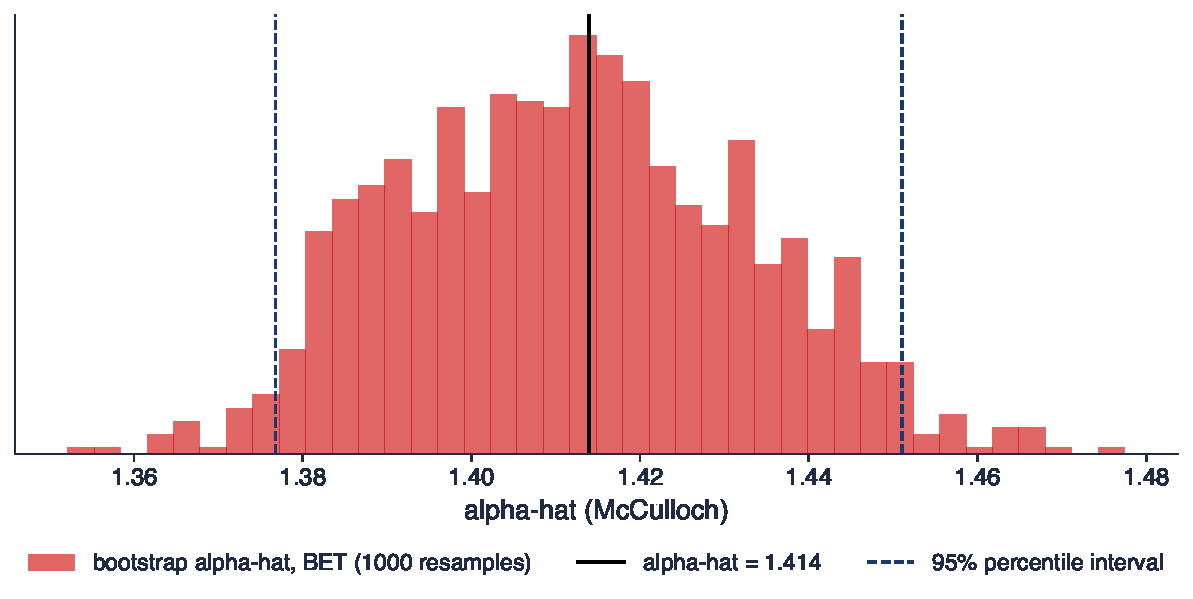
\includegraphics[width=0.96\textwidth,height=0.42\textheight,keepaspectratio]{ch3_sem_b1.pdf}
\end{center}
\vspace{-2mm}
\begin{itemize}
    \item $n = 6\,670$; cuantile $-1{,}93$, $-0{,}50$, $0{,}08$, $0{,}66$, $2{,}06$; $\nu_\alpha = 3{,}425$, $\nu_\beta = -0{,}006$
    \item $\hat\alpha = 1{,}414$, $\hat\beta = -0{,}011$, $\hat\gamma = 0{,}60\%$, $\hat\delta_0 = 0{,}079\%$; SE bootstrap $0{,}021$, interval de 95\% $[1{,}377; 1{,}451]$
    \item Interpretare: $\alpha = 2$ este mult în afara intervalului; corpul și cozile BET sînt mult mai largi decît permite distribuția Normală
\end{itemize}\quantlet{SFM\_ch3\_seminar}{\qlurl{SFM_ch3_seminar}}
\end{frame}

\begin{frame}{B2: încă trei piețe [Propus]}
\itemsize{\footnotesize}
\begin{itemize}
\item \textbf{Întrebarea}: care dintre S\&P 500, DAX și Bitcoin are cele mai groase cozi după metoda McCulloch? Model: B1.
\item \textbf{Date}: S\&P 500 și DAX din 2000, Bitcoin din 2014, randamente logaritmice zilnice în \%
\item \textbf{Cerințe}
\begin{enumerate}
    \item Repetați pașii 1--3 din B1 pentru fiecare serie.
    \item Puneți $\nu_\alpha$, $\hat\alpha$ cu intervalul lui, $\hat\beta$ și $\hat\gamma$ pentru cele patru serii (cu BET) într-un tabel.
    \item Interpretare: este diferența dintre $\hat\alpha$ al Bitcoin și cel al S\&P 500 mai mare decît eroarea de estimare?
\end{enumerate}
\item \textbf{Raportați}: un tabel și două fraze
\item Notebook: secțiunea B2
\end{itemize}
\end{frame}

\ifsolutions
\begin{frame}{B2: rezolvare [Propus]}
\itemsize{\footnotesize}
\begin{center}
\footnotesize
\begin{tabular}{lrrrrr}
\toprule
& $\nu_\alpha$ & $\hat\alpha$ & interval 95\% & $\hat\beta$ & $\hat\gamma$ (\%) \\
\midrule
BET & $3{,}425$ & $1{,}414$ & $[1{,}377; 1{,}451]$ & $-0{,}011$ & $0{,}60$ \\
S\&P 500 & $3{,}338$ & $1{,}438$ & $[1{,}396; 1{,}475]$ & $-0{,}151$ & $0{,}54$ \\
DAX & $3{,}285$ & $1{,}455$ & $[1{,}416; 1{,}506]$ & $-0{,}113$ & $0{,}68$ \\
Bitcoin & $3{,}803$ & $1{,}322$ & $[1{,}275; 1{,}369]$ & $-0{,}027$ & $1{,}44$ \\
\bottomrule
\end{tabular}
\end{center}
\begin{itemize}
    \item Cele mai groase cozi: Bitcoin, $\hat\alpha = 1{,}322$; intervalul lui nu se suprapune cu cel al S\&P 500
    \item BET, S\&P 500 și DAX: intervale care se suprapun, fără un clasament clar
    \item $\hat\gamma$ al Bitcoin este de peste două ori mai mare decît cel al indicilor
\end{itemize}\quantlet{SFM\_ch3\_seminar}{\qlurl{SFM_ch3_seminar}}
\end{frame}
\fi

\begin{frame}{B3: verosimilitate maximă pentru S\&P 500 [Rezolvat]}
\itemsize{\scriptsize}
\begin{itemize}
\item \textbf{Întrebarea}: descrie ajustarea stabilă ML randamentele S\&P 500 mai bine decît distribuția Normală, în corp și în cozi?
\item \textbf{Date}: închiderile S\&P 500 din 2000, randamente logaritmice zilnice în \%
\item \textbf{Cerințe}
\begin{enumerate}
    \item Ajustați legea stabilă prin ML (S0) și raportați $\hat\alpha$ și $\hat\beta$ cu erorile standard, $\hat\gamma$, $\hat\delta_0$ și $\hat\delta_1$.
    \item Comparați $\hat\alpha$ cu estimarea McCulloch.
    \item Ajustați distribuția Normală și distribuția Student-t și comparați AIC (Akaike information criterion, criteriul informațional Akaike, $2k - 2\ell$) al celor trei modele.
    \item Desenați graficul QQ al datelor față de ajustările Normală și stabilă.
    \item Interpretare: unde eșuează fiecare model?
\end{enumerate}
\item \textbf{Raportați}: estimările, trei valori AIC, graficul QQ și două fraze
\item Notebook: secțiunea B3
\end{itemize}
\end{frame}

\begin{frame}{B3: rezolvare [Rezolvat]}
\itemsize{\scriptsize}
\begin{center}
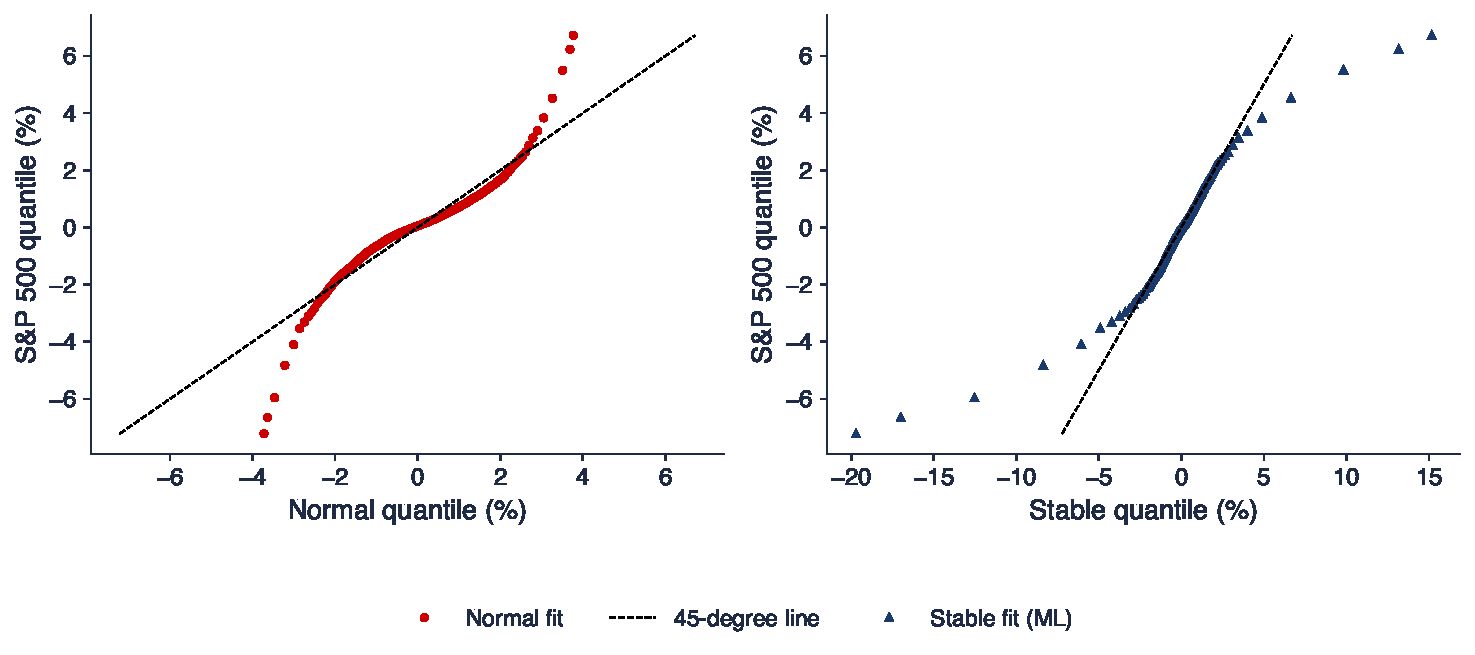
\includegraphics[width=0.96\textwidth,height=0.40\textheight,keepaspectratio]{ch3_sem_b3.pdf}
\end{center}
\vspace{-2mm}
\begin{itemize}
    \item ML: $\hat\alpha = 1{,}540$ (SE $0{,}021$, CI 95\% $[1{,}499; 1{,}581]$), $\hat\beta = -0{,}181$ ($0{,}036$), $\hat\gamma = 0{,}58$, $\hat\delta_0 = 0{,}093$, $\hat\delta_1 = 0{,}000$; McCulloch $\hat\alpha = 1{,}438$
    \item AIC: Normală 21\,650, Student-t 19\,702, stabilă 19\,794: legea stabilă bate distribuția Normală la 1\,856 de puncte, Student-t bate legea stabilă la 92 de puncte
    \item Interpretare: ajustarea Normală ratează cozile (cuantila de 0,1\% $-3{,}72$ vs $-7{,}22$ în date); ajustarea stabilă le depășește ($-19{,}70$)
\end{itemize}\quantlet{SFM\_ch3\_seminar}{\qlurl{SFM_ch3_seminar}}
\end{frame}

\begin{frame}{B4: pierderi mari Bitcoin în trei modele [Propus]}
\itemsize{\scriptsize}
\begin{itemize}
\item \textbf{Întrebarea}: care model reproduce cel mai bine numărul pierderilor zilnice mari ale Bitcoin? Model: B3.
\item \textbf{Date}: închiderile Bitcoin din 2014, 7 zile pe săptămînă, randamente logaritmice zilnice în \%
\item \textbf{Cerințe}
\begin{enumerate}
    \item Ajustați legile Normală, Student-t și stabilă (ML).
    \item Numărați zilele cu o pierdere peste 10\% și peste 20\%.
    \item Calculați numărul așteptat de astfel de zile în fiecare model, $n \times P(r < -x)$.
    \item Calculați VaR 1\% al datelor și al fiecărui model.
    \item Interpretare: ce model ați folosi pentru o cerință de marjă pe o poziție în Bitcoin și de ce?
\end{enumerate}
\item \textbf{Raportați}: un tabel de numărători, patru valori VaR și două fraze
\item Notebook: secțiunea B4
\end{itemize}
\end{frame}

\ifsolutions
\begin{frame}{B4: rezolvare [Propus]}
\itemsize{\footnotesize}
\begin{center}
\footnotesize
\begin{tabular}{lrrrr}
\toprule
& observat & Normală & Student-t & stabilă \\
\midrule
pierdere peste 10\% (zile) & 56 & $8{,}1$ & $54{,}2$ & $73{,}9$ \\
pierdere peste 20\% (zile) & 4 & $\approx 0$ & $12{,}3$ & $26{,}9$ \\
VaR 1\% (\%) & $10{,}5$ & $8{,}0$ & $11{,}1$ & $14{,}3$ \\
\bottomrule
\end{tabular}
\end{center}
\begin{itemize}
    \item $n = 4\,384$; stabilă ML: $\hat\alpha = 1{,}410$ ($0{,}026$), $\hat\beta = 0{,}019$, $\hat\gamma = 1{,}54$; Student-t $\hat\nu = 2{,}23$
    \item Normală: mult prea puține pierderi mari; stabilă: prea multe peste 20\%; Student-t: cea mai apropiată la 10\%, prea multe la 20\%
    \item Interpretare: Student-t sau legea stabilă ca limită prudentă; niciodată distribuția Normală
\end{itemize}\quantlet{SFM\_ch3\_seminar}{\qlurl{SFM_ch3_seminar}}
\end{frame}
\fi

\begin{frame}{B5: rămîne $\alpha$ la fel cînd randamentele se adună? [Rezolvat]}
\itemsize{\footnotesize}
\begin{itemize}
\item \textbf{Întrebarea}: dacă randamentele zilnice S\&P 500 ar fi i.i.d.\ stabile, randamentele săptămînale și lunare ar avea același $\alpha$; îl au?
\item \textbf{Date}: randamentele logaritmice zilnice S\&P 500 din 2000; sumele săptămînale și lunare
\item \textbf{Cerințe}
\begin{enumerate}
    \item Calculați randamentele logaritmice săptămînale și lunare ca sume ale celor zilnice.
    \item Calculați $\hat\alpha$ McCulloch la cele trei orizonturi.
    \item Faceți bootstrap pentru fiecare $\hat\alpha$ cu 500 de reeșantionări și raportați intervalele de 95\%.
    \item Interpretare: este tiparul compatibil cu randamente stabile i.i.d.?
\end{enumerate}
\item \textbf{Raportați}: trei estimări cu intervale, graficul și două fraze
\item Notebook: secțiunea B5
\end{itemize}
\end{frame}

\begin{frame}{B5: rezolvare [Rezolvat]}
\itemsize{\footnotesize}
\begin{center}
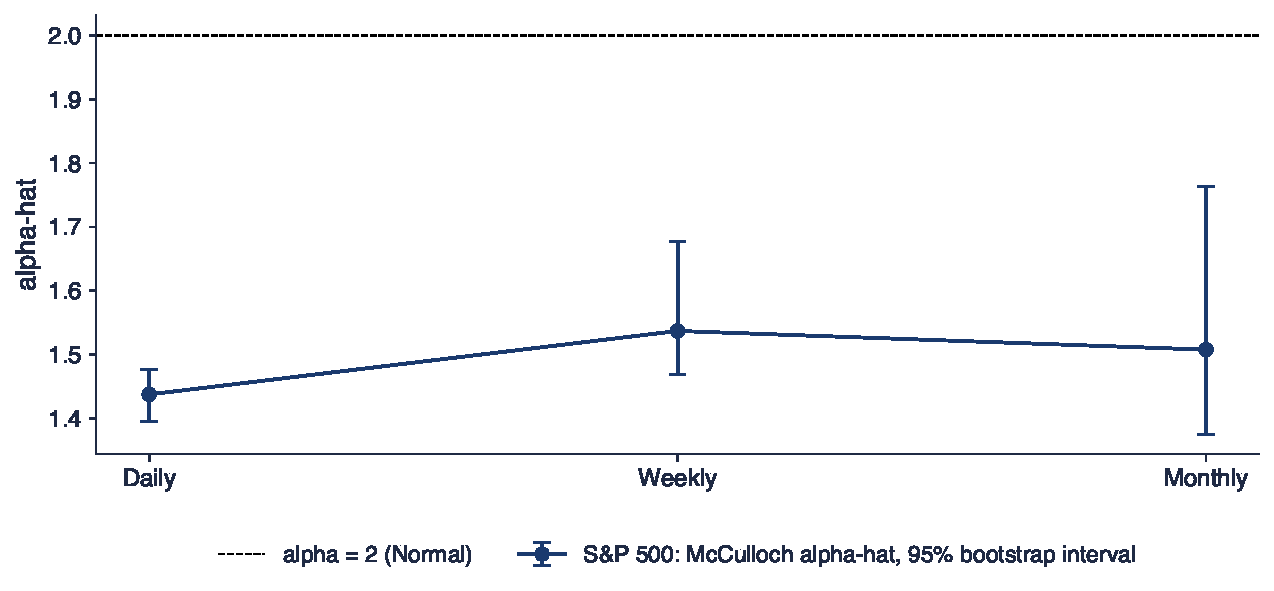
\includegraphics[width=0.96\textwidth,height=0.42\textheight,keepaspectratio]{ch3_sem_b5.pdf}
\end{center}
\vspace{-2mm}
\begin{itemize}
    \item Zilnic ($n = 6\,714$): $1{,}44$ $[1{,}40; 1{,}48]$; săptămînal ($1\,394$): $1{,}54$ $[1{,}47; 1{,}68]$; lunar ($321$): $1{,}51$ $[1{,}37; 1{,}76]$
    \item $\hat\alpha$ este mai mare pentru randamentele săptămînale decît pentru cele zilnice; intervalul lunar este larg și urcă pînă la $1{,}76$
    \item Interpretare: un $\alpha$ crescător este un semnal împotriva randamentelor stabile i.i.d.; eșantioanele lunare sînt prea scurte pentru un răspuns ferm (Cursul 3 repetă testul cu ML)
\end{itemize}\quantlet{SFM\_ch3\_seminar}{\qlurl{SFM_ch3_seminar}}
\end{frame}

\begin{frame}{B6: se stabilizează varianța de selecție? [Propus]}
\itemsize{\footnotesize}
\begin{itemize}
\item \textbf{Întrebarea}: este varianța de selecție a randamentelor BET și Bitcoin atît de mare și de instabilă cît implică o lege stabilă cu $\alpha$ estimat? Modele: B1, B5.
\item \textbf{Date}: BET din 2000, Bitcoin din 2014, randamente logaritmice zilnice în \%
\item \textbf{Cerințe}
\begin{enumerate}
    \item Calculați varianța de selecție a fiecărei serii pe tot eșantionul și pe prima jumătate.
    \item Simulați 200 de traiectorii de aceeași lungime din ajustarea McCulloch (CMS) și calculați varianța de selecție a fiecărei traiectorii.
    \item Raportați mediana și percentilele de 5\% și 95\% ale varianțelor simulate, precum și proporția celor sub varianța observată.
    \item Interpretare: ce spune comparația despre ipoteza varianței infinite?
\end{enumerate}
\item \textbf{Raportați}: un tabel cu două rînduri și o frază
\item Notebook: secțiunea B6
\end{itemize}
\end{frame}

\ifsolutions
\begin{frame}{B6: rezolvare [Propus]}
\itemsize{\footnotesize}
\begin{center}
\footnotesize
\begin{tabular}{lrrrrrr}
\toprule
& $\hat\alpha$ & var. date & prima jumătate & mediana sim. & sim. 5--95\% & proporția sub \\
\midrule
BET & $1{,}414$ & $2{,}0$ & $3{,}0$ & $19{,}2$ & $[7{,}3; 215{,}0]$ & $0\%$ \\
Bitcoin & $1{,}322$ & $12{,}1$ & $15{,}4$ & $213{,}0$ & $[63{,}2; 4442{,}0]$ & $0\%$ \\
\bottomrule
\end{tabular}
\end{center}
\begin{itemize}
    \item Varianța observată este sub toate varianțele simulate: randamentele reale sînt mult mai puțin extreme decît implică legea stabilă ajustată
    \item Interpretare: dovezi împotriva varianței infinite; varianța primei jumătăți diferă de cea a eșantionului complet pentru că volatilitatea se schimbă în timp
\end{itemize}\quantlet{SFM\_ch3\_seminar}{\qlurl{SFM_ch3_seminar}}
\end{frame}
\fi


%=============================================================================
\section{Partea C: întrebări deschise și critica unui răspuns AI}
%=============================================================================

\begin{frame}{C1: este $\alpha$ constant în timp? [Propus]}
\itemsize{\footnotesize}
\begin{itemize}
\item \textbf{Întrebarea}: se schimbă cozile BET și S\&P 500 de la o perioadă de cinci ani la alta?
\item \textbf{Date}: randamente logaritmice zilnice din 2000, împărțite în 2000--2004, 2005--2009, 2010--2014, 2015--2019, 2020--2026; modele: B1, B3
\item \textbf{Cerințe}
\begin{enumerate}
    \item Calculați $\hat\alpha$ McCulloch cu un interval bootstrap în fiecare perioadă, pentru fiecare indice.
    \item Spuneți care perioade diferă semnificativ.
    \item Propuneți o explicație a schimbărilor și o cale de a o testa (de exemplu, randamente împărțite la o volatilitate mobilă).
    \item Interpretare: ce ar însemna un $\alpha$ variabil pentru un model de risc estimat pe date vechi?
\end{enumerate}
\item \textbf{Raportați}: un tabel, o scurtă listă de schimbări semnificative și un plan de proiect
\item Notebook: secțiunea C1
\end{itemize}
\end{frame}

\ifsolutions
\begin{frame}{C1: analiză de referință [Propus]}
\itemsize{\scriptsize}
\begin{center}
\scriptsize
\begin{tabular}{llrrr}
\toprule
Indice & perioada & $n$ & $\hat\alpha$ & interval 95\% \\
\midrule
BET & 2000--2005 & 1238 & $1{,}46$ & $[1{,}38; 1{,}58]$ \\
BET & 2005--2010 & 1245 & $1{,}48$ & $[1{,}40; 1{,}59]$ \\
BET & 2010--2015 & 1261 & $1{,}52$ & $[1{,}42; 1{,}64]$ \\
BET & 2015--2020 & 1251 & $1{,}64$ & $[1{,}51; 1{,}81]$ \\
BET & 2020--2026 & 1675 & $1{,}48$ & $[1{,}43; 1{,}58]$ \\
S\&P 500 & 2000--2005 & 1254 & $1{,}63$ & $[1{,}50; 1{,}77]$ \\
S\&P 500 & 2005--2010 & 1258 & $1{,}28$ & $[1{,}23; 1{,}39]$ \\
S\&P 500 & 2010--2015 & 1258 & $1{,}42$ & $[1{,}35; 1{,}50]$ \\
S\&P 500 & 2015--2020 & 1257 & $1{,}35$ & $[1{,}28; 1{,}43]$ \\
S\&P 500 & 2020--2026 & 1687 & $1{,}54$ & $[1{,}45; 1{,}65]$ \\
\bottomrule
\end{tabular}
\end{center}
\begin{itemize}
    \item S\&P 500: $\hat\alpha$ între $1{,}28$ și $1{,}63$, cel mai mic în 2005--2010 (criza financiară globală); mai multe intervale nu se suprapun
    \item BET: între $1{,}46$ și $1{,}64$; schimbările urmează regimurile de volatilitate, un semn al grupării volatilității (Capitolul 9)
    \item Direcții de proiect: ferestre mobile, ML, randamente standardizate cu volatilitatea GARCH, mai multe acțiuni BVB
\end{itemize}\quantlet{SFM\_ch3\_seminar}{\qlurl{SFM_ch3_seminar}}
\end{frame}
\fi

\begin{frame}{C2: verificați un răspuns AI [Propus]}
\itemsize{\scriptsize}
\begin{itemize}
    \item Un student a cerut unui asistent AI să ajusteze o lege stabilă pe randamentele logaritmice zilnice S\&P 500 (\%) din 2000. Răspunsul:
    \item \aiprompt{(a) levy\_stable din scipy folosește implicit S0, deci loc = 0{,}000 este locația S0 delta0.}
    \item \aiprompt{(b) Cu alpha = 1{,}540 și gamma = 0{,}58, varianța randamentelor zilnice este 2 gamma\textasciicircum 2 = 0{,}68.}
    \item \aiprompt{(c) Scala randamentelor pe 20 de zile este sqrt(20) x gamma = 2{,}60\%.}
    \item \aiprompt{(d) Deoarece alpha < 2, VaR 1\% al acestui model nu există.}
    \item \aiprompt{(e) Deoarece alpha > 1, randamentul zilnic mediu există.}
    \item Cerințe
    \begin{itemize}
        \item 1. Pentru fiecare afirmație spuneți dacă este corectă; dacă nu, dați afirmația corectă și, unde se poate, cifra corectă din notebook (secțiunea C2).
        \item 2. Raportați: o listă de cinci verdicte, fiecare cu un rînd de justificare.
    \end{itemize}
\end{itemize}
\end{frame}

\ifsolutions
\begin{frame}{C2: rezolvare [Propus]}
\itemsize{\footnotesize}
\begin{itemize}
    \item (a) Greșit: scipy folosește implicit S1; $\hat\delta_1 = 0{,}000$ și $\hat\delta_0 = \hat\delta_1 + \hat\beta\hat\gamma\tan\frac{\pi\hat\alpha}{2} = 0{,}093$
    \item (b) Greșit: $2\gamma^2$ este varianța doar pentru $\alpha = 2$; cu $\alpha < 2$, varianța modelului este infinită; varianța de selecție este $1{,}47$
    \item (c) Greșit: în modelul stabil, scala crește ca $20^{1/\alpha}$: $6{,}99 \times 0{,}58 = 4{,}07\%$, nu de $\sqrt{20} = 4{,}47$ ori
    \item (d) Greșit: cuantilele există întotdeauna; VaR 1\% al legii stabile ajustate este $4{,}54\%$ (ES este cel care cere $\alpha > 1$, ceea ce este adevărat aici)
    \item (e) Corect: $E|X| < \infty$ pentru că $1 < \alpha$; în S1, media este egală cu $\delta_1$
\end{itemize}\quantlet{SFM\_ch3\_seminar}{\qlurl{SFM_ch3_seminar}}
\end{frame}
\fi


%=============================================================================
\section{Încheiere}
%=============================================================================

\begin{frame}{Ce rămîne de azi}
\itemsize{\small}
\begin{itemize}
    \item O sumă stabilă de $n$ termeni se scalează ca $n^{1/\alpha}$, mai repede decît $\sqrt{n}$ cînd $\alpha < 2$
    \item Cunoașteți parametrizarea: S0 și S1 diferă prin locație; scipy folosește S1
    \item McCulloch: cinci cuantile și un tabel; ML: mai precisă; bootstrap pentru intervale
    \item Randamentele reale: $\hat\alpha$ mult sub 2 la orizont zilnic, dar varianța se stabilizează, iar $\hat\alpha$ crește prin agregare
    \item Un răspuns AI este o ciornă: verificați parametrizarea, regula scalei și ce există pentru $\alpha < 2$
\end{itemize}
\end{frame}

\begin{frame}{După seminar}
\itemsize{\small}
\begin{itemize}
    \item Cursul 3 dezvoltă fiecare temă de azi: stabilitatea, CLT generalizată, parametrii, cozile, simularea, estimarea și critica
    \item Încercați cerințele [Propus] în notebook; rezolvările se discută la seminar
    \item C1 poate deveni un proiect de echipă: ferestre mobile, ML, mai multe piețe
    \item Lectură: \refNolan, cap.~1; \refBHW; \refMcCulloch
\end{itemize}
\end{frame}


%=============================================================================
\section{Bibliografie}
%=============================================================================

\begin{frame}{Bibliografie}
\itemsize{\tiny}
\begin{itemize}
    \item Borak, S., Härdle, W., Weron, R. (2005). \href{https://doi.org/10.1007/3-540-27395-6_1}{Stable distributions}. In Čížek, P., Härdle, W., Weron, R. (eds.), \textit{Statistical Tools for Finance and Insurance}, 21--44. Springer.
    \item Chambers, J.M., Mallows, C.L., Stuck, B.W. (1976). \href{https://doi.org/10.1080/01621459.1976.10480344}{A method for simulating stable random variables}. \textit{Journal of the American Statistical Association}, 71(354), 340--344.
    \item Franke, J., Härdle, W.K., Hafner, C.M. (2019). \href{https://doi.org/10.1007/978-3-030-13751-9}{\textit{Statistics of Financial Markets: An Introduction}}, 5th ed. Springer.
    \item Mandelbrot, B. (1963). \href{https://doi.org/10.1086/294632}{The variation of certain speculative prices}. \textit{Journal of Business}, 36(4), 394--419.
    \item McCulloch, J.H. (1986). \href{https://doi.org/10.1080/03610918608812563}{Simple consistent estimators of stable distribution parameters}. \textit{Communications in Statistics -- Simulation and Computation}, 15(4), 1109--1136.
    \item Nolan, J.P. (2001). \href{https://doi.org/10.1007/978-1-4612-0197-7_17}{Maximum likelihood estimation and diagnostics for stable distributions}. In Barndorff-Nielsen, O.E., Mikosch, T., Resnick, S.I. (eds.), \textit{Lévy Processes}, 379--400. Birkhäuser.
    \item Nolan, J.P. (2020). \href{https://doi.org/10.1007/978-3-030-52915-4}{\textit{Univariate Stable Distributions: Models for Heavy Tailed Data}}. Springer.
    \item Weron, R. (1996). \href{https://doi.org/10.1016/0167-7152(95)00113-1}{On the Chambers--Mallows--Stuck method for simulating skewed stable random variables}. \textit{Statistics \& Probability Letters}, 28(2), 165--171.
\end{itemize}
\end{frame}

\end{document}
